\section{DEFINING SPECIALIZED CYBER RED TEAM RESPONSIVE OPERATIONS}
\label{sec:crtopreq}
\glsresetall
Nations are not well known to announce publicly their offensive cyber capacities and more focused on advertising and promoting cyber defence activities and initiatives. Despite this, the identified major cyber intelligence programmes attributed to nation states, such as, US NSA PRISM\footnote{The Verge. ``Everything you need to know about PRISM.'' \url{https://www.theverge.com/2013/7/17/4517480/nsa-spying-prism-surveillance-cheat-sheet}. Accessed: 28/09/2018} and UK GCHQ TEMPORA\footnote{Wired. ``A simple guide to GCHQ's internet surveillance programme Tempora.'' \url{https://www.wired.co.uk/article/gchq-tempora-101}. Accessed: 28/09/2018}, prove to represent the actual cyber capabilities of some NATO alliance members.
Also, collective defence alliances and treaties as of now do not acknowledge cyber offence as a collective approach and leave such initiatives up to every individual nation to assess and develop on its own. However, this does not exclude any other allies either requesting such assistance or joining forces to engage in offensive cyber operations.
Furthermore, responsive cyber defence balances between the defensive and offensive posture and can enable defenders to engage the adversary both in their own cyber infrastructure, as well as globally. However, there is no clear understanding on how such activities can be executed and what their operational and technical requirements are.

This chapter addresses responsive activities taken in the cyberspace by introducing and defining the concept of \textit{specialized cyber red team responsive computer network operations}. This concept is divided into three main components: 1) responsive cyber defence -- the overarching concept defining the defender's posture to pursue the adversary to ensure the maximum possible protection of the defended assets; 2) computer network operations -- are the means of the defender to exercise this posture against the adversary and systems engaged in the attack; and 3) cyber red team -- the actual team of experts possessing the required skills and capabilities to engage in such responsive operations.

The following subsections present the individual concepts of responsive cyber defence, computer network operations, cyber red teaming, and assesses their minimal operational requirements.
These principles lay the required foundation to define, once combined, the specialized cyber red team responsive operations and specify their requirements.

\subsection{Responsive Cyber Defence Requirements}
\label{sec:rcd}
\glsresetall
% RCD definition
\gls{rcd} is a controversial, vaguely understood and seldom used term. More commonly, a broader concept of \gls{acd} is utilized as presented in chapter \ref{sec:rcd-work}.
One definition states that \gls{acd} is accomplished through denial to information and deception via misleading information \cite{Heckman2013} \cite{Heckman2015}.
Another definition suggests actively engaging the incoming cyber attack to destroy or reduce its effectiveness \cite{Denning2014}, or conduct the hack-back \cite{Mansfield2009}.
Contrary to this, US DARPA acknowledges \gls{acd} (see footnote \ref{fnote:darpa} on page \pageref{fnote:darpa}) without the component of actively pursuing and interacting with the adversary.
Yet another \gls{acd} concept is directed to threat assessment and mitigation \cite{Dewar2017}.
Some view this approach purely limited to one set of approaches (e.g. \textit{``white worms''}, address hopping) \cite{Lu2013} \cite{Repik2008}.
One proposed \gls{rcd} definition is aimed at gaining access to the third-party systems for modification or deletion of data held therein \cite{Maybaum2014}.
Another \gls{rcd} definition is quite broad and permits any applicable defensive actions to be taken against any communication and information system engaged or used in the attack \cite{Brangetto2014-2}.
These various definitions of \gls{acd} are mainly focused towards the integrated and synchronized real-time capability for detection, analysis, identification, and mitigation aimed at degrading or eliminating the adversary offensive capacity.
Tackled \gls{acd} activities do not necessarily limit the response to be expanded beyond the defender's own systems, however, they are still primarily focused towards combating the adversary and its activities within the defended networks and information systems.

% ACD definition weaknesses and RCD definition.
The aforementioned definitions for the \gls{rcd} already address a more targeted response, going beyond one's own infrastructure, and by actively pursuing the perpetrators through other information systems and networks. The concepts addressed in these definitions are limited in scope and do not include the principle of system monitoring, information gathering or alteration of system behaviour to allow further intelligence gathering and attribution. Such responsive actions should at all times grant the situational awareness and permit collection of information for the responding \gls{crt}. Such properties are crucial to allow defenders to trace the cyber attack back to its origin.
This thesis addresses the various interpretations and concepts of active and responsive cyber defence and defines the responsive cyber defence.
\begin{description}
    \label{def:rcd}
    \item \textbf{Definition 1.} Responsive cyber defence is a responsive activity (1) exercised by conducting cyber operations (2) against engaged external information systems (3) to defend own information systems (4).

    With the essential elements of the definition being:
    \begin{enumerate}
        \item response to an incoming threat, which can be executed in real-time as the attack commences or asynchronously once enough attribution information is gathered. The incoming attack against the defended information systems is the main precondition for engaging in \gls{rcd};
        \item cyber operations, such as, computer network operations as discussed in chapter \ref{sec:cno};
        \item the extraterritorial nature of \gls{rcd} means that the exercised activities are directed either against adversary's or third-party information systems, which are being used by the attacker. Within this thesis, information system\footnote{The Information system definition derived from author's personal experience merged with Encyclopaedia Britannica definition of Information System. \url{https://www.britannica.com/topic/information-system}. Accessed: 11/11/2018} is understood as a set of information technologies, software, physical infrastructure, human resources, procedures and regulations, used for creating, storing and processing information belonging to and governed by a certain entity; and
        \item the measures required for ensuring the protected system defence, which include the activities, such as, attack detection, identification, analysis, threat assessment, and attribution, aimed at destroying or reducing the effectiveness of the attack.
    \end{enumerate}
\end{description}

% RCD applicability
It has to be noted, that \gls{rcd}, in contrast to \gls{acd}, can only be executed in case of a verified attack or directed aggression. The \gls{rcd} per se is not pre-emptive but can be exercised as a subset within a broader responsive encounter, such as, political or kinetic, which in turn can be pre-emptive.
As such, the \gls{rcd} capability does not have to be constantly active or exposed as it would be in case of a more permanent \gls{acd} techniques, for example, deceptions and honeypots. Such responsive capabilities would be maintained, kept at high readiness level and alert, but activated only once the circumstances necessitate either within the \gls{acd} scope or independently.
The Fig.\ref{fig:acdrcd} illustrates the relation between the \gls{acd} and \gls{rcd} to represent the scope of engagement, dependencies and applicability.
As shown, the \gls{rcd} is oriented at engagements beyond own infrastructure, however, still heavily depending on the initial detection, analysis and identification capability provided either by the deployed threat detection solutions or \gls{acd} techniques. To reach the defined goals of the \gls{rcd}, the \gls{crt} would have to trace back the intrusion through the attack paths, which would include the global communication infrastructure owned by the \gls{isp} or unwitting third-party networks. Additionally, taking control or delivering the desired impact to the perpetrator's deployed attack infrastructure, which could consist of digital and physical assets set up or compromised by the attacker.
Extraterritorial nature of \gls{rcd} means that other engaged or involved parties, such as, proxies and breached public services to host the malware or \gls{cnc}, can be targeted by the responders to trace back or affect the capabilities or paths taken by the attackers. This property of \gls{rcd}, as well as \gls{acd}, is heavily discussed and tackled by the legal experts \cite{Brangetto2014-2}. Despite implied legal ramifications, this thesis focuses purely on the technical approaches and methods, by providing only a brief insight into the associated legal concerns (see section \ref{sec:scenario} on page \pageref{sec:scenario}).
The \gls{crt} would operate and conduct the \gls{cno} from its own created and built infrastructure separated from the defended network. Due to this, the \gls{crt} has to maintain all the capabilities to continuously detect, identify, analyse and assess the threats while executing the \gls{cno} within the \gls{rcd}. This means, the \gls{crt} has to persistently follow the principle implied by the \gls{ooda} loop\footnote{US Defense Technical Information Center. \url{http://www.dtic.mil/docs/citations/ADA566700} Accessed: 11/11/2018} to maintain the visibility of the ongoing activities and keep track on the perpetrator movement, actions, origin and presence. However, in this thesis, a fully functional capability and developed operational network is assumed and is not tackled in a greater detail regarding such operational network design, asset procurement, deployment, modification, and destruction, as it is out of the scope of this work. However, some insight in operational network structure prototyping and defence is given in chapter \ref{sec:protection}.

\begin{figure}[!htb]
    \centering
    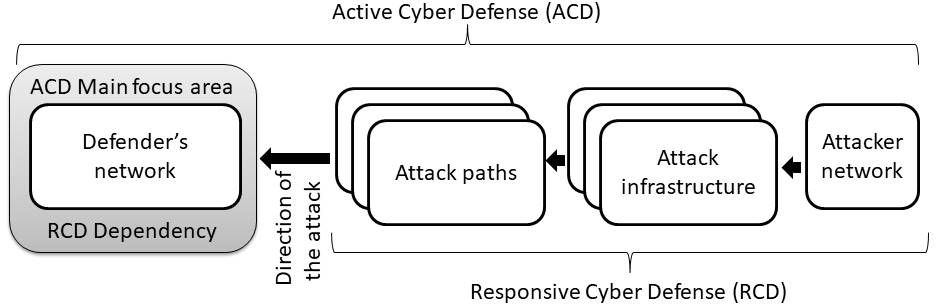
\includegraphics[width=0.8\textwidth]{./img/acd-rcd.jpg}
    \caption{Active and responsive cyber defence areas of engagement}
    \label{fig:acdrcd}
\end{figure}

% RCD requirements
Based on the related work, as presented in the chapter \ref{sec:rcd-work} and discussed here, the \gls{rcd} has at least the following requirements and characteristics:
\begin{enumerate}
    \item \textbf{Available.} The capability has to be permanently maintained and ready for deployment at the shortest notice possible.
    \item \textbf{Coordinated.} Has to be in response to an verified aggression and coordinated between the responders at various directions, such as, political, kinetic, or \gls{cnd}.
    \item \textbf{Integrated.} Compliant with the initial threat detection, assessment, and related \gls{acd} activities.
    \item \textbf{Synchronized.} Real-time as the attack has been detected and is still ongoing. Additionally, it can be asynchronous in cases when the attack has seized, but the artefacts have been identified through activities, such as, vulnerability assessment, threat hunting, digital forensics, or signature update on the threat detection and analysis systems.
    \item \textbf{Automated.} Maximum automation to allow the highest level of synchronization and minimize the time required for the early stages of response.
    \item \textbf{Asymmetric.} Every \gls{crt} action has to deliver the maximum possible effect. Which correlates with the high readiness and preparedness level of the \gls{crt}.
    \item \textbf{Omnipresent.} Ability to track and pursue adversary throughout the cyberspace with the highest flexibility possible.
    \item \textbf{Effective.} Capable of delivering the required impact, such as, destroy or reduce effectiveness of the attack, engage adversary by denial \& deception or a hack-back.
    \item \textbf{Independent.} \gls{crt} has to contain all the necessary capabilities to conduct the \gls{rcd}.
\end{enumerate}
This is not an exhaustive list and more characteristics could be applicable depending on the particular \gls{rcd} specifics and delivered effect requirements.
\subsection{Computer Network Operation Requirements}
\label{sec:cno}
\glsresetall
% CNO definition
The \gls{cno} definition varies from the perspective and the tier of applicability, such as, political, strategic or tactical, as presented in chapter \ref{sec:cno-work}.
The US doctrine encompasses the computer network operations as a set of various activities within the computer networks \cite{Leblanc2011} or employment of cyberspace capabilities to achieve objectives in or through the cyberspace \cite{USJCS2018}.
One definition offers to treat the cyber operations as a manoeuvre in cyberspace to apply force to achieve a position or advantage in the cyber domain \cite{Applegate2012}.
Another view point states, that \gls{cno} is always offensive in nature and is of a dual use \cite{Robinson2015}.
Furthermore, it is inclined, that such cyber operations can be exclusively exercised only within cyber warfare and military engagements \cite{Dewar2017}.
These definitions are mainly focused towards various activities, either defensive or offensive, performed by the use of computer networks, and define the \gls{cno} appropriately.

% CNO definition weaknesses and re-definition
The inconclusiveness brought by few of the definitions regarding \gls{cno} being limited to cyber warfare is unclear and restrictive on the applicability of this concept.
This thesis addresses the various \gls{cno} interpretations and defines computer network operations.
\begin{description}
    \label{def:cno}
    \item \textbf{Definition 2.} Computer network operations are any set (1) of effect-oriented activities (2) performed by the application of force (3) in the cyberspace by the use of computer networks (4).

    With the essential elements of the definition being:
    \begin{enumerate}
        \item single or a group of activities supporting either each other, having a common direction or aimed at reaching same effect by various means in cyberspace;
        \item instead of being limited to an explicit set of predefined activities, an effect-based approach is considered. The desired effect is specified by the operational requirements or aligned with the supported operation demands. Such activities can include, for example, defensive, responsive, offensive, intelligence, or information operations;
        \item application of force constitutes to specifically directed and focused activities against the elements of the target information system; and
        \item the use of computer networks, to achieve the desired operational effect in cyberspace, is the main feature and pre-condition for such operations. It can be a hybrid approach, where the computer network operation delivers one effect in cyberspace with an intention to trigger the desired effects, such as, kinetic or impacting the adversary decision-making process.
    \end{enumerate}
\end{description}

% CNO applicability
The \gls{cno} concept can include any subset of activities utilizing computer networks, such as, \gls{cnd}, \gls{cne}, or \gls{cna}. Within this scope, by \gls{cne} is understood the offensive use of computer networks to conduct target information system infiltration activities, for example, executing cyber espionage or cyber reconnaissance operations. The \gls{cnd} and \gls{cna} are more specific, and each encapsulates purely either the defensive or offensive nature of the computer network use. A responsive \gls{cno} is an operation executed within the \gls{rcd}. These activities do not have to be limited just to these particular tasks and any type of operation, as long as it is dependent on computer networks, can be applicable to \gls{cno}. For example, cyber espionage operation, relying on \gls{cne} to access and apply \gls{cna} to gain position in the target network, would also be considered as a \gls{cno}. The operation, as the term implies, is oriented towards delivering effects by application of force in the cyberspace and is not to be confused with a regular use computer networks and their services, such as, browsing the Internet or accessing e-mail. From this perspective, the \gls{cno} can carry any desired effect, either again cyber or physical, to be delivered by the means of computer networks, such as, offensive, disruptive, denial, or deceptive.
These concepts are represented in Fig.\ref{fig:cno} from the perspective of peace- and war-time, \gls{acd}, \gls{rcd} and cyber warfare paradigms. The \gls{rcd} is an overarching measure, consolidating all of the operation types applicable to both war and peace. The author argues, that in the current political era, it is becoming harder to distinguish the peace- and war-time operations since the thresholds in cyberspace are becoming more obscure as the nation-states practice more unconventional and hybrid warfare.

\begin{figure}[!htb]
    \centering
    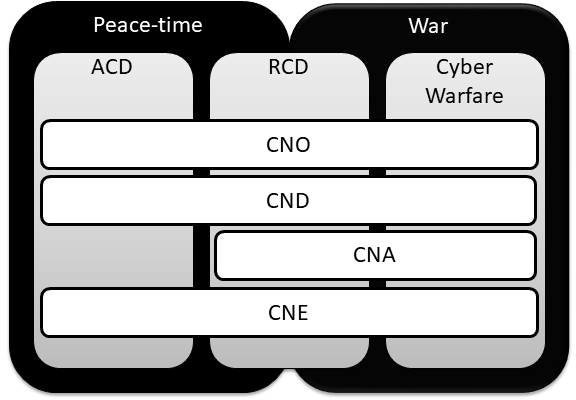
\includegraphics[width=0.5\textwidth]{./img/cno.jpg}
    \caption{Computer network operation applicability to operational paradigms}
    \label{fig:cno}
\end{figure}

% CNO requirements
Based on the related work, as presented in the chapter \ref{sec:cno-work} and discussed here, the \gls{cno} has at least the following requirements and characteristics:
\begin{enumerate}
    \item \textbf{Hybrid.} \gls{cno} can be used to aid both defensive and offensive effects as well as any other activities in support for achieving these effects.
    \item \textbf{Rapid.} Ability to deliver fast paced operation execution if such capability is prepared and maintained.
    \item \textbf{Focused.} Possibility to achieve rapid concentration of force in cyberspace on single or a small set of targets.
    \item \textbf{Dynamic.} Capability to adjust, evolve, and mutate according to the changing environment and operational needs to provide inconsistency.
    \item \textbf{Agile.} Possesses high manoeuvrability supported by the dynamic nature.
    \item \textbf{Stealthy.} Granting limited attribution, protection of identity and privileges.
    \item \textbf{Pervasive.} Has long operational reach and can target any interconnected node remotely in the cyberspace to provide access and control.
    \item \textbf{Parallel and distributed.} Can be launched from multiple sources in the cyberspace simultaneously against a single or a set of targets.
    \item \textbf{Effective.} Has the potential capability of delivering cyber and, if designated -- kinetic effects.
    \item \textbf{Asymmetric.} Can deliver higher operational effect in contrast to other operations, if prepared and used accordingly.
\end{enumerate}
This is not an exhaustive list and more characteristics could be applicable depending on the particular \gls{cno} specifics.
\subsection{Cyber Red Teaming Requirements}
\label{sec:crt}
\glsresetall
% CRT definition
The \gls{rt} definition varies on the domain to which this capability is applied, such as -- command, military, or cyber, as it is discussed in the chapter \ref{sec:crt-work}.
Most common \gls{rt} definition revolves around a small, independent team of highly skilled experts, to provide decision support, alternative analysis and approaches to an existing problem \cite{UK2013} \cite{USJCS2016}.
One definition attempts to present military \gls{crt} as an adversarial-based assessment of own information system vulnerabilities \cite{Brangetto2015}.
Additionally, \gls{rt} is seen as a decision-making supportive element for conducting asymmetric warfare \cite{Longbine2008}.
These definitions are more focused towards supporting decision-making process or providing a specialized assessment of own assets in cyberspace or physically.
It has to be noted, that the \gls{crt} is the \gls{rt} utilizing and performing their assigned tasks mainly within cyberspace and by the use of technology.

% CRT definition weaknesses and re-definition
The aforementioned definitions are directed towards securing and evaluating defender's systems or course of action, but not at affecting the adversary's information systems or decision-making process.
To engage a \gls{crt} in conducting a \gls{cno} within the \gls{rcd} scope, which has the extraterritorial nature, the \gls{crt} has to be structured and possess all the defined qualities and high standards of the \gls{rt}. However, to separate the \gls{rt} activities between internal and external, a concept of \textit{``specialized cyber red teaming''}, directed at the adversary, is proposed.
This thesis addresses the various red team interpretations, use cases, and their applicability, and defines the specialized cyber red team.
\begin{description}
    \label{def:crt}
    \item \textbf{Definition 3.} specialized cyber red team is an independent team of highly skilled experts (1) tasked to perform activities (2) against the adversary's cyber capabilities (3).

    With the essential elements of the definition being:
    \begin{enumerate}
        \item a fully functional and self-sustainable cyber red team operating within the cyberspace;
        \item timely and focused activities against the adversary, for example, conducting the adversarial vulnerability assessment, capability and \gls{tttp} analysis, or execution of computer network operations; and
        \item the cyber red team performed activities being in support of decision-making process, ongoing related operations, or having its own impact delivery.
    \end{enumerate}
\end{description}

% SpecCRT applicability
Such \gls{crt} would be tasked to operate on its own or deliver an effect in support of other activities, such as, cyber-kinetic engagements.
\gls{crt} as such retains the capabilities to operate at any level applicable to deliver the required effect. This could mean operating through kinetic and cyber means to deliver the impact, either directly or indirectly, on the target's cyber or kinetic assets, as long as the execution of operation has the cyber component (Fig. \ref{fig:crt}). As an example, a \gls{crt} might engage in social engineering campaign to gain access to a target server room either physically (e.g., acquiring or copying access cards) or via cyber means (e.g., obtaining remote access password). As well as, for example, gaining remote access to a adversary server room \gls{hvac} system and shutting it down to cause physical effects or damage.
As for the \gls{rt} adversary and threat emulation principle, the \gls{crt} may exercise these approaches to conduct a \textit{false-flag} or \textit{no-flag} operations. Within such operations, the \gls{crt} would pretend and assume the role of another threat actor and adopt its \gls{tttp} to confuse the enemy and make attribution harder or force it to be incorrect.
It has to be pointed out, that the \gls{crt} is a team with suggested size of no more than ten highly skilled experts to keep it balanced and agile, as it is proposed by the UK doctrine \cite{UK2013}. Such small team requires every participant to assume multiple roles to support all of the \gls{crt} operational needs, such as, operational infrastructure planning and deployment, asset acquire, intelligence gathering, \gls{opsec} assurance, targeting, monitoring, and own asset protection. Depending on the available resources and goals, a separate team can be established to support all of the \gls{crt} operational requirements.
Most importantly, a specialized \gls{crt} is the perfect candidate for executing a \gls{cno} within the scope of \gls{rcd}, hence, combining all of the requirements, benefits and restrictions. To create, develop, maintain and evolve such a complete capability the proper resources have to be allocated and invested as early as possible. However, in this thesis, a fully functional specialized \gls{crt} is assumed, and no deeper insights are provided on the assembly, management and its operational requirements, as it is out of the scope of this work.

\begin{figure}[!htb]
    \centering
    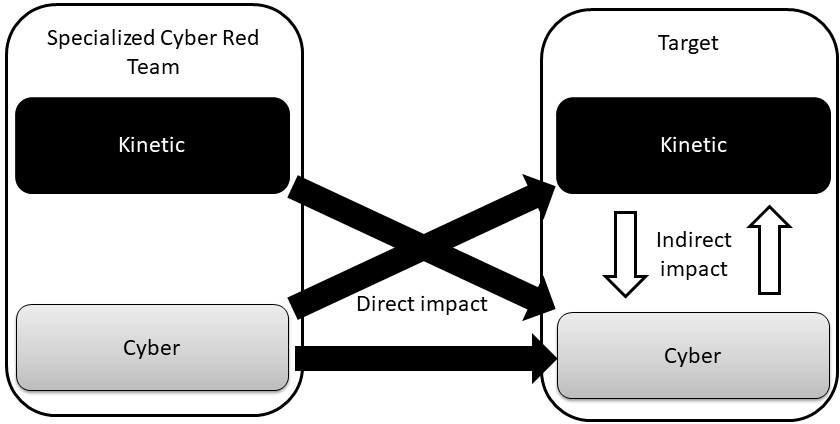
\includegraphics[width=0.8\textwidth]{./img/scrt.jpg}
    \caption{Special cyber red team operation effects}
    \label{fig:crt}
\end{figure}

% CRT requirements
Based on the related work, as presented in the chapter \ref{sec:crt-work} and discussed here, the \gls{crt} has at least the following requirements and characteristics:
\begin{enumerate}
    \item \textbf{Small.} A small team of experts for increased ease of management and agility.
    \item \textbf{Skilled.} Every expert has to be skilled to contribute to the \gls{crt} capability.
    \item \textbf{Specialized.} The team has to self-sustain its independence and operational requirements by providing all the necessary specialized skills.
    \item \textbf{Innovative.} Finding alternative approaches and identifying vulnerabilities in the designated target systems or processes, by applying creativity, critical review and thinking techniques.
    \item \textbf{Highly focused.} Aimed at conducting a specific operation to deliver the designated effect.
    \item \textbf{Targeted.} Persistent in performing precision strikes to complete the assigned task.
    \item \textbf{Asymmetric.} A small team with highly skilled experts having the capability on delivering the maximum possible effect.
    \item \textbf{Adaptive.} Adapting and employing adversarial \gls{tttp} against the target system.
    \item \textbf{Supportive.} Providing support to the ongoing operations, decision-making processes, and operation planning.
    \item \textbf{Timely.} Has to deliver the required effects in the defined time frame.
\end{enumerate}
This is not an exhaustive list and more characteristics could be applicable depending on the particular \gls{crt} organization and tasking specifics.


\section{SPECIALIZED CYBER RED TEAM RESPONSIVE OPERATIONS}
\label{sec:crtops}
\glsresetall
Concepts, methods and approaches presented in the listed publications (\ref{pub:firstPub}, \ref{pub:secondPub}, and \ref{pub:thirdPub}) are applied to fulfil the requirements of specialized cyber red team responsive cyber operations, allowing the creation of custom cyber red team tools and techniques for the responsive operation execution. Furthermore, such technique applicability is evaluated and proposed to counter the cyber kill-chain. Additionally, an insight into legal ramifications of specialized cyber red team responsive operations is presented.

\subsection{Operational Requirements}
\label{sec:scrtop}
\glsresetall
The requirements listed separately for \gls{rcd}, \gls{cno}, and \gls{crt} have to be combined to define the demands of the specialized cyber red team responsive computer network operations, as it consolidates all of the individual concepts. The techniques and tools, presented in the listed publications, are described and mapped against these criteria to identify how they can benefit, enhance and support the \gls{tttp} creation for specialized \gls{crt} responsive \gls{cno} fulfilment.

% DEFINITION
\begin{description}
    \label{def:scrtop}
    \item \textbf{Definition 4.} Specialized cyber red team responsive computer network operations are such computer network operations (1), which are executed by a specialized cyber red team (2) within the responsive cyber defence (3).

    With the essential elements of the definition being:
    \begin{enumerate}
        \item computer network operations according to Definition 2 on page \pageref{def:cno};
        \item specialized cyber red team according to Definition 3 on page \pageref{def:crt}; and
        \item responsive cyber defence according to Definition 1 on page \pageref{def:rcd}.
    \end{enumerate}
\end{description}

\begin{table}[!htb]
\centering
\resizebox{\textwidth}{!}{%
\begin{tabular}{|l|p{1.5cm}|l|p{2cm}|c|c|c|}
\hline
\textbf{RCD} & \textbf{CNO}             & \textbf{CRT} & \textbf{Specialized CRT Responsive CNO}     & \textbf{Pub.I} & \textbf{Pub.II} & \textbf{Pub.III} \\ \hline
Independent  &                          & Skilled      & \multirow{4}{2.2cm}{Stealthy and innovative}& \multirow{4}{*}{X}     & \multirow{4}{*}{X}      & \multirow{4}{*}{X}       \\ \cline{1-3}
             &                          & Specialized  &                                             &                        &                         &                          \\ \cline{1-3}
             & Dynamic                  & Adaptive     &                                             &                        &                         &                          \\ \cline{1-3}
             & Stealthy                 & Innovative   &                                             &                        &                         &                          \\ \hline
Available    & Agile                    & Small        & Agile and available                         & X                      & X                       &                          \\ \hline
             & Focused                  & Focused      & Focus of force                              &                        & X                       & X                        \\ \hline
Omnipresent  & Pervasive                & Targeted     & \multirow{2}{2.2cm}{Targeted and pervasive} & \multirow{2}{*}{X}     & \multirow{2}{*}{X}      & \multirow{2}{*}{X}       \\ \cline{1-3}
             & Parallel and distributed &              &                                             &                        &                         &                          \\ \hline
Automated    &                          &              & \multirow{2}{2.2cm}{Rapid and timely}       & \multirow{2}{*}{}      & \multirow{2}{*}{X}      & \multirow{2}{*}{}        \\ \cline{1-3}
Synchronized & Rapid                    & Timely       &                                             &                        &                         &                          \\ \hline
Integrated   &                          &              & \multirow{2}{2.2cm}{Integrated and coordinated} & \multirow{2}{*}{}  & \multirow{2}{*}{}       & \multirow{2}{*}{X}       \\ \cline{1-3}
Coordinated  &                          & Supportive   &                                             &                        &                         &                          \\ \hline
             & Hybrid                   &              & \multirow{2}{2.2cm}{Hybrid and effective}   & \multirow{2}{*}{}      & \multirow{2}{*}{X}      & \multirow{2}{*}{X}       \\ \cline{1-3}
Effective    & Effective                &              &                                             &                        &                         &                          \\ \hline
Asymmetric   & Asymmetric               & Asymmetric   & Asymmetric                                  &                        & X                       & X                        \\ \hline
\end{tabular}%
}
\caption{Specialized CRT responsive CNO grouping and TTTP mapping to publications}
\label{tab:scrt}
\end{table}

The table \ref{tab:scrt} represents the features of every individual \gls{rcd}, \gls{cno} and \gls{crt} concept grouped to form the specialized cyber red team responsive computer network operation requirements. These requirements are then mapped against the methods and approaches presented in the publications to introduce \gls{tttp} supporting this objective. In the table, the `X' denotes that a particular technique, presented in that publication, is applicable to the specialized cyber red team responsive operation specific technique, tool and procedure development. The listed techniques are not exhaustive and do not form a complete list, but represent the ones as introduced in the listed publications.
At least the following characteristics are applicable to the proposed new concept:
\begin{enumerate}
    \item \textbf{Stealthy and innovative.} Grasps the core requirements for self-sustainability, evolution and adjustment to the changing environment, adaptation of adversarial \gls{tttp}, independence and innovative skills, to provide the maximum possible level of stealth and make attribution harder;
    \item \textbf{Agile and available.} A prepared and on demand available, small team with high manoeuvrability;
    \item \textbf{Focus of force.} Allows achieving rapid concentration of force focused on performing a specific operation against a single or a small set of targets in the cyberspace;
    \item \textbf{Targeted and pervasive.} Is specifically crafted and designed to deliver the required single impact or a set of parallel activities remotely from any position in the cyberspace;
    \item \textbf{Rapid and timely.} Enabling the fast and automated execution of synchronized activities in the designated time or against the adversary as the ongoing attack progresses;
    \item \textbf{Integrated and coordinated.} Support to other responsive operations and activities in a coordinated manner based on initial threat assessment;
    \item \textbf{Hybrid and effective.} Can be applicable both to defensive or offensive activities, delivering required impact against kinetic or cyber assets; and
    \item \textbf{Asymmetric.} Has to provide maximum possible effect with minimum available resources against a stronger adversary.
\end{enumerate}
This is not an exhaustive list and it can be expanded or optimized with the characteristics, which could be applicable depending on specific operational goals, desired effects and available resources.


\subsection{Techniques, Tools, Tactics and Procedures}
\label{sec:ttps}
The techniques and tools presented in listed publications are logically intertwined to provide the support for the cyber red team operation key stage execution. Those being -- gaining initial access (\ref{pub:secondPub}), establishing a command and control channel (\ref{pub:firstPub}), and delivering the impact (\ref{pub:thirdPub}). These critical stages are part of nearly any cyber operation (see table \ref{tab:achain} on page \pageref{tab:achain}), where the network perimeter needs to be breached to establish initial foothold (e.g., through cyber means or kinetic to cyber methods), a secure channel is required to provide path into the target system for lateral movement and asset location, and finally the designated impact delivery. Every computer network operation will have its own requirements and effects to be delivered to the adversary information systems. In some cases, to deliver the desired effect, the cyber components are just means of triggering it, such as, disabling the power to force the use of backup generator, conduct a \gls{dos} to compel to switch to insecure communication lines, target the integrity of a military command and control system to degrade situational awareness and cause incorrect decision-making.
The following sections, in a structured way, review the publications and present the fundamental techniques, prototyped tools, and procedures for technique and tool applicability to the specified cyber red team operation requirements (see table \ref{tab:scrt}).


\subsubsection{Gaining Initial Access}
\label{sec:access}
\textbf{Techniques.}
\ref{pub:secondPub} shows the novel and easy to use method for binary protocol bit-aware fuzzing and reverse-engineering \cite{Blumbergs2017}.
The core concepts introduced by that work rely on creative way for atomic data manipulation exposing vulnerabilities and attack vectors.
Assessed network protocol fuzzing frameworks are limited to fuzzing one byte as the smallest unit of data. Such limitation to one byte can be reasonable when assessing the protocols located at the upper layers of the OSI model, such as, FTP, HTTP, and DNS. However, this is a severely limiting factor restricting binary protocol analysis and fuzzing, where the data fields can be of a variable length and not always compatible with a length of one byte. For example, the IPv6 header Flow Label field is 20 bits long and cannot be byte-aligned to comply with the protocol specification. In essence, nearly any network communication protocol can be treated as ``binary protocol'' since they are composed of multiple variable length bit groups (i.e., bit-fields). The proposed solution accepts one bit as the smallest unit of data, thus allowing flexible fuzzing test-case creation. This permits practically any communication protocol analysis independent of its OSI layer, such as, performing Layer-2 Ethernet frame or Layer-3 IP packet fuzzing. The proposed technique is also applicable to other media, such as, serial line communications, as long as available hardware and software supports it. In the conducted experiments a proprietary serial line protocol ported to TCP/IP stack was successfully targeted.

In general, fuzzing does not immediately guarantee to find exploitable vulnerabilities, since this depends on multiple factors, such as, targeted software development quality, complexity, used programming language, code coverage, test-case correctness, and time. The assessed popular fuzzing frameworks have a complex targeted protocol description and test-case creation process.
\textit{Bbuzz} attempts to ease this process, speed-up the increased quality test-case creation, and minimize time investment for attack set-up through systematic and easy to use approach.

\textbf{Tools.}
Based on these principles, the \textit{Bbuzz} framework for systematic binary protocol fuzzing and reverse-engineering is prototyped, described and applied in practice by the author to confirm its applicability and value for cyber red team operations.
This framework allows an automated test-case generation by analysing the available sample traffic and applying methods, such as, bit-group pattern matching, mutable and immutable field identification, and entropy measurements. Such approach, in case of available traffic capture, allows a rapid initial test-case generation and start of the fuzzing process. For effective test-case generation the framework uses various field mutation approaches and produces n-fold Cartesian product of all available payload field mutation sets. This ensures that all possible payload combinations from individual field mutation sets are generated to grant the most complete set of test-cases.

The table \ref{tab:fuzz} briefly summarizes the findings from \ref{pub:secondPub} to compare the commonly used fuzzing frameworks and tools against the developed \textit{Bbuzz} framework (tools are listed in \textbf{bold} in the table). The comparison criteria is based on the following requirements (listed in \textit{italics} in the table): open-source and available on demand to the \gls{crt} depending on the operational requirements; reasonably maintained by the developers to ensure it being up to date as much as possible; is designed or can be applied to support also network protocol fuzzing; can fuzz the protocol starting from OSI Layer-2; the fuzzing test-cases support variable length bit-fields, which can be fuzzed bit-wise with one bit being the smallest fuzzing test-case; can be used to perform network traffic sample analysis to identify features, such as, pattern mining, immutable and mutable bit-field identification, and field Shannon entropy calculations; based on the traffic analysis can automatically create the initial test case; and can monitor the target system under test as much as it is possible depending on the use case. In the table, the field marked with \textit{'Yes'} denotes, that this feature is supported, and \textit{'No'} presents the lack of support for the respective framework. Target monitoring for \textit{Taof} has been labelled as \textit{'Partial'} since the tool expects a reply from the target system and if it is not received, then an exception is assumed. Multiple features for the \textit{Afl} have been marked as \textit{'Partial'} since it is a file format based fuzzer, but can be used to generate test cases from a sample network packet, which have to be wrapped by other means to be sent over the network to the destination. \textit{Bbuzz} is aimed at remote system testing over network and supports ICMP echo messages and port probing to detect a possible exception condition, therefore it has been labelled as \textit{'Partial'}. From the presented results it can be observed, that the \textit{Bbuzz} tool can deliver more flexibility and functional diversity for the \gls{crt} when compared to other common fuzzing frameworks.

\begin{table}[!htb]
\centering
\resizebox{\textwidth}{!}{%
\begin{tabular}{|l|l|l|l|l|l|l|l|l|}
\hline
                                                                           & \textbf{Spike} & \textbf{Sulley} & \textbf{Boofuzz} & \textbf{Peach CE} & \textbf{Taof} & \textbf{Zzuf} & \textbf{Afl} & \textbf{Bbuzz} \\ \hline
\textit{Open-source}                                                       & Yes            & Yes             & Yes              & Yes               & Yes           & Yes           & Yes          & Yes            \\ \hline
\textit{Maintained}                                                        & No             & No              & Yes              & Yes               & No            & Yes           & Yes          & Yes            \\ \hline
\textit{Network-based}                                                     & Yes            & Yes             & Yes              & Yes               & Yes           & Yes           & No           & Yes            \\ \hline
\textit{Layer-2}                                                           & No             & No              & No               & No                & No            & No            & Partial      & Yes            \\ \hline
\textit{Bit-wise}                                                          & No             & No              & No               & No                & No            & No            & Partial      & Yes            \\ \hline
\textit{\begin{tabular}[c]{@{}l@{}}Traffic sample\\ analysis\end{tabular}} & No             & No              & No               & No                & No            & No            & Partial      & Yes            \\ \hline
\textit{\begin{tabular}[c]{@{}l@{}}Automatic\\ test-cases\end{tabular}}    & No             & No              & No               & No                & No            & No            & Partial      & Yes            \\ \hline
\textit{\begin{tabular}[c]{@{}l@{}}Target\\ Monitoring\end{tabular}}       & No             & Yes             & Yes              & Yes               & Partial       & No            & No           & Partial        \\ \hline
\end{tabular}%
}
\caption{Common fuzzing framework comparison to \textit{Bbuzz}}
\label{tab:fuzz}
\end{table}

As a use case, \textit{Bbuzz} was applied to quickly reverse-engineer key features of the NATO proprietary Link-1 binary protocol, which is used for real-time air picture representation at the military operations centres and air traffic control stations. The protocol property reverse-engineering, such as, flight number, coordinates, altitude, bearing, velocity, and \gls{iff} code, allowed the injection of fake aeroplane tracks via the computer network. This attack vector was used to degrade the situational awareness and decision-making process of a NATO operation, performed within the NATO response force readiness exercise STEADFAST COBALT 2017\footnote{SHAPE. ``Exercise Steadfast Cobalt set to get underway in Lithuania.'' \url{https://shape.nato.int/news-archive/2017/exercise-steadfast-cobalt-set-to-get-underway-in-lithuania}. Accessed 23/09/2018}.
The \textit{Bbuzz}\footnote{Bbuzz. \url{https://github.com/lockout/Bbuzz}. Accessed: 01/10/2018} framework, written in Python 3, has been released publicly on GitHub under the MIT license and is freely available to everyone for usage and further customization.

Additionally, the published work had the following impact on the international security community:
Link-1 attacks were implemented in the game network of the NATO CCD CoE executed \gls{cdx} ``Locked Shields 2017'' and successfully executed by the \gls{crt} against defending \textit{Blue Team} systems;
enhanced discussions at NATO Communications and Information Agency (NCIA) on accelerating the Link-1 protocol revision and its long-term deprecation plans;
as well as further applicability for \gls{ics}/\gls{scada} protocol reverse-engineering and attacks \cite{Blumbergs2018};
and generating malicious traffic for testing the unsupervised framework for detecting anomalous Syslog messages \cite{Vaarandi2018}.

\textbf{Tactics and procedures.}
It has to be noted, that vulnerability identification and exploit development can be a lengthy and tedious task, however, the cyber red team tool-set, such as, \textit{Bbuzz}, provides the necessary means to ease, automate and deliver results faster. Though the approach not being stealthy in its nature, it gives the innovative way on finding targeted vulnerabilities in the adversary's information systems and developing custom exploits, which will raise the level of stealth and increase operational success.
For this to be possible either an initial intelligence information is required or the reconnaissance needs to be performed. Intelligence information provided either by the intelligence service or collected by the red team through open source intelligence (OSINT) will give a starting position on understanding if such technique and tools are applicable to achieving this goal. If the operational and time constraints allow and this is deemed as a valid option to be pursued, then further data might be required. Additional information, depending on the target exposure could be collected via the means of active (e.g., network port scans, banner grabbing) or passive (e.g., using online solutions such as \textit{Shodan}, or any other applicable OSINT technique) reconnaissance. The gathered information would allow the cyber red team to attempt to replicate the target system in a controlled and closed testing environment.
Targeting software and communication protocols via methods, such as, fuzzing, can be applicable throughout the cyber red team attack life-cycle to find vulnerabilities or ways on how to otherwise abuse the target under test.

From the perspective of custom exploit development for the initial adversary network targeting to gain the foothold, this can be seen as one of the valid options for stealthy network entry. Especially favoured in case when traditional entry methods, such as, \textit{spear-phishing} campaign or known exploit execution might be not desired as they could raise attention and trigger alerts. As well as, in cases when the external network services have limited attack surface and only few options to attempt remote attacks are viable.
To attempt such an attack, the initial information is preferred well in advance due to time requirements for reference system creation, vulnerability identification, and exploit verification. However, fuzz-testing can be integrated in any phase of activity to explore alternative ways while pursuing ready-available attacks paths, since it is always available and relatively easy and fast to be set-up.

Such focus of force on one or small set of targets for finding vulnerabilities has its risks and benefits. Investing resources in finding a targeted vulnerability in a small set of services, instead of attempting on finding attack vectors in every exposed asset, has to be well assessed from the perspective of sensibility of attack, likelihood of possible flaws and expertise required to transform them into functioning exploit. However, in a successful case such attack vector can be a significant asset when executing computer network operations or assisting other related activities. Not only support to achieving the initial foothold can be obtained but depending on the possible and desirable effects also other direct or indirect impact can be inflicted on both the cyber and kinetic components. Not always the targeted element of the system is the intended target, but it can serve as an indirect mean to accomplish the desired effect, such as, obscuring adversary's situational awareness. 
Taking into consideration all the aforementioned limitations and advantages, the successfully identified custom vulnerability will grant a small cyber red team a higher success of operation execution.

The presented and verified concepts and approaches contribute to the following operational requirement development:
stealthy and innovative,
agile and available,
focus of force,
targeted and pervasive,
rapid and timely,
effective, and
asymmetric.


\subsubsection{Establishing Command and Control Channel}
\label{sec:cnc}
\textbf{Techniques.}
\ref{pub:firstPub} presents the novel and simple ways for covert channel creation based on IPv6 transition technologies \cite{Blumbergs2016}.
The fundamental approaches are based on innovative and creative use of existing technology present in current computer networks.
The covert channel creation approach relies on IPv6 transition mechanisms, such as, dual-stack, encapsulation and tunnelling. These technologies exist in vast majority of current computer networks and are supported by nearly all network communication devices and operating systems. Based on this, it is possible, for example, to create an egress covert channel from the dual stack network, where network engineers have implemented IPv4 addressing scheme, but are not controlling the IPv6, either because not being aware of it or not having a full understanding on how to properly implement, control and secure it. One method uses the IPv4 as a transport layer to establish an IPv6 connectivity by the means, such as, \textit{6in4} encapsulation or \gls{gre} tunnelling. Additionally, for a dual-stack network, it is possible to establish multiple simultaneous IPv4 and IPv6 connections to various destination IP addresses and exfiltrate data over those. As verified in the experiment, the \gls{nids} would not be able to establish the context, correlate the packets and perform analysis which are split and sent over IPv4 and IPv6 in a randomly selected order. This happens because two different IP stacks are used for packet delivery and tested \gls{nids} solutions do not treat such split packets as belonging to the same network data stream. This was identified as a fundamental flaw in the \gls{nids} implementations requiring their redesign and detection algorithm remodelling.

\textbf{Tools.}
Based on these principles, two tools -- \textit{tun64} and \textit{nc64}, are prototyped, described and thoroughly tested by the author and a team of anomaly and intrusion detection experts. Tests are performed against a set of commercial and open-source solutions, such as, \textit{Snort}, \textit{Suricata}, \textit{Bro}, and \textit{Moloch}. The commercial tools are not mentioned explicitly due to discretion and vendors not agreeing to allow their names to be announced, however, among those are the market leaders for \gls{ids}, \gls{nids} and \gls{dlp} products. Prototyped attack tools are tested alongside with other common covert channel creation techniques, such as, HTTP, DNS, ICMP, SSH and \textit{netcat} based tunnels, running on applicable and various common TCP and UDP ports. In a conducted experiment, the proposed approaches are verified to be capable of successfully bypassing the \gls{nids} detection and allowing covert channel establishment to be used for various purposes, such as, \gls{cnc} channel establishment and data exfiltration. Furthermore, the \textit{nc64} tool has been successfully implemented into the cyber red team tool-set for data exfiltration and attack execution against the defending blue teams within the largest international live-fire technical cyber defence exercise ``Locked Shields''.
Both prototyped tools\footnote{tun64. \url{https://github.com/lockout/tun64}. Accessed: 01/10/2018} \footnote{nc64. \url{https://github.com/lockout/nc64}. Accessed: 01/10/2018}, written in Python, are publicly released on GitHub under the MIT license and available to be used by everyone.

The table \ref{tab:tun} represents a shortened and condensed version of findings from \ref{pub:firstPub} related to developed tool \textit{nc64} and \textit{tun64} comparison to other commonly used protocol tunnelling method (represented in \textit{italics} in the table) detection by popular open-source monitoring, \gls{nids}, and \gls{dpi} solutions (represented in \textbf{bold} in the table). The chosen monitoring tools are \textit{Snort} \gls{nids} with Source Fire (SF) and Emerging Threats (ET) signatures, Suricata \gls{nids}, \textit{Bro} and \textit{Moloch} \gls{dpi} solutions. The tested popular commercial \gls{nids} and \gls{dpi} solutions are not listed or mentioned due to signed non-disclosure agreements, however, the prototyped approaches were able to circumvent the detection with high success ratio.
The listed tool configuration notation follows the following convention \textit{tool\_name-transport\_protocol-port-IPversion(s)}, for example, the \textit{nc64} tool running over TCP to a destination port 80 using IPv6 and IPv4 interchangeably would be written as \textit{nc64-t-80-6/4}.
The test outcomes are labelled as follows: a positive match (denoted by letter Y in the table) clearly identified a malicious activity and triggered alerts, partial or abnormal footprint (denoted by letter P) raised the alert but did not provide appropriate information, potential visible match (denoted by letter V) requires human analyst or sophisticated anomaly detection for a positive match verification, and the worst case (denoted by letter N) does not generate any visible alerts or logs. From the presented results it can be seen, that the \textit{nc64} tool is successful on evading the implemented automated threat detection solutions and has a higher evasion success rate than other protocol tunnelling methods, as well as, it has not been fingerprinted in comparison to the well-known \textit{netcat} tool.

\begin{table}[!tb]
\centering
\begin{tabular}{|l|l|l|l|l|l|}
\hline
                            & \textbf{Snort SF} & \textbf{Snort ET} & \textbf{Suricata} & \textbf{Bro} & \textbf{Moloch} \\ \hline
\textit{http-t-80-4}        & N                 & N                 & V                 & V            & V               \\ \hline
\textit{iodine-u-53-4}      & N                 & N                 & Y                 & P            & V               \\ \hline
\textit{ptunnel-icmp}       & N                 & Y                 & N                 & V            & V               \\ \hline
\textit{netcat-t-80-6}      & N                 & N                 & N                 & V            & N               \\ \hline
\textit{ssh-t-80-6}         & N                 & N                 & V                 & P            & N               \\ \hline
\textit{tun64-t-80-t6over4} & N                 & Y                 & Y                 & P            & N               \\ \hline
\textit{nc64-t-80-6/4}      & N                 & N                 & N                 & P            & V               \\ \hline
\textit{nc64-t-443-6}       & N                 & N                 & N                 & V            & N               \\ \hline
\end{tabular}
\caption{Common tunnelling method detection comparison to \textit{nc64} and \textit{tun64}}
\label{tab:tun}
\end{table}

Furthermore, these techniques support target system remote access from nearly any location in the cyberspace. Major global initiatives executed by the global standardization and industry leaders, such as, ``World IPv6 Day'', are accelerating the introduction of IPv6 throughout the Internet with its backbone already being fully IPv6 but lagging at the network edges. To support the IPv6 connectivity for the IPv4 networks, the transition mechanisms are introduced and maintained until the Internet has fully migrated to IPv6. Widespread deployment and availability of IPv6 and required transition mechanisms make this attack approach, as implemented in the \textit{nc64} and \textit{tun64}, global and available throughout the cyberspace. Furthermore, it can be assumed, that IPv4 enabled networks with transition mechanisms enabled will remain for an undefined period of time.

Additionally, the published work had the following impact on the international security community:
EUROPOL European Cybercrime Centre (EC3) released a security warning on IPv6 vulnerabilities \cite{EC3-2017-7};
Forum of Incident Response and Security Teams (FIRST) annual conference sparked discussions on IPv6 security\footnote{FIRST Conference 2018. F.Herberg, SWITCH. \url{https://www.first.org/resources/papers/conf2018/Herberg-Frank_FIRST_20180624.pdf}. Accessed: 23/09/2018};
IETF discussions on protocol specification updates and transition mechanism deprecation (private e-mail exchange between the IETF representatives and the author);
NIDS vendor system updates (private e-mail exchange between the vendor and the author);
and multiple news articles\footnote{InfoSecurity. ``NATO CCDCoE: IPv6 Transition Opens Up Covert Info Exfiltration.'' \url{https://www.infosecurity-magazine.com/news/nato-ipv6-transition-opens-up/}. Accessed: 23/09/2018} \footnote{Slashdot. ``Tunnelled IPv6 Attacks Bypass Network Intrusion Detection Systems.'' \url{https://tech.slashdot.org/story/17/04/09/0452220/tunnelled-ipv6-attacks-bypass-network-intrusion-detection-systems}. Accessed: 23/09/2018}.

\textbf{Tactics and procedures.}
The implemented tools and approaches provide high level of flexibility and usage applicability since they are built on top of a network protocol stack supported by nearly all modern network devices and operating systems. Such capability yields to the cyber red team with extra level of stealth due to readily-available technology use in the modern computer networks. Both the \textit{tun64} and \textit{nc64} tools are applicable to achieving this goal, however, \textit{nc64} showing better results in circumventing network security solutions. Since the \textit{tun64} amd \textit{nc64} tools, alongside with the automated testing network creation scripts, have been publicly released, they are freely available for the cyber red team to be used for any tailored access operations.

The main area of such technique applicability is for maintaining control over the compromised assets in the target network, either in the first stages of the attacks or when moving laterally in the network and searching for the intended target. Such created \gls{cnc} channels permit not only the control over the specific systems, but also any other data exchange, such as valuable data exfiltration. Furthermore, when engaging in lateral movement within the dual-stack network such approach can be used to maintain the desired level of stealth. This can be accomplished either by moving from one compromised host to another by the means of such techniques, or interconnecting internal network nodes to create a path which is harder to be traced back to its origin and initial entry point. When targeting multi-tiered networks such as \gls{ics}/\gls{scada}, consisting of various in-depth network segments, maintaining a stable \gls{cnc} channel is of a high priority to deliver the designated impact to the target systems.

Detecting such implemented covert channel was identified to be extremely hard, even by a human analyst, since there were no known patterns or signatures to be matched against the large volume of data collected by the \gls{dpi}. The common \gls{cnc} channels would rely on using typical protocols such as DNS, HTTP, and within the MS Windows network -- SMB, to carry the data in the protocol payload fields. These approaches are well known to the analysts, even if the covert method is not known. If the IPv6 transition mechanism based covert channel is implemented properly, such as, network port aligned with its expected payload headers (e.g., HTTP headers over TCP/80), then the chances of remaining undetected are increasing. This consideration is applicable to any other technique used by cyber red team, for example, when targeting or impersonating a particular network service, the performed activities have to comply with at least the expected patterns of timing, network protocol, source and destination ports, and protocol payload main features.
From the conducted experiments, it was identified, that the prototyped \textit{nc64} tool had the best detection evasion indicators when using the following ports -- UDP/22, TCP/443, UDP/443, and UDP/80.
The presented and verified concepts and approaches contribute to the following operational requirement development: stealthy and innovative, agile and available, and targeted and pervasive. 


\subsubsection{Delivering the Impact}
\label{sec:impact}
\textbf{Techniques.}
\ref{pub:thirdPub} displays the novel and automated approaches for \gls{ics}/\gls{scada} protocol, system takeover and process control \cite{Blumbergs2018}.
The basic ideas represented in this work are vulnerability location methods, verification and weaponization for critical impact infliction.
Utilizing these approaches, the \gls{ics}/\gls{scada} network protocols -- PROFINET IO and IEC-104, dominantly used in European automation and power grids, were reverse-engineered by the author and approaches for malicious command injection developed. The described attack vectors, explained by \gls{poc} code, were exploited to successfully compromise the industrial and electrical power grid process. The techniques of identifying such attack vectors and exploiting them rely primarily on the protocols lacking the security features. Even if security mechanisms exist, such as, IEC-104 security extensions they are seldom implemented by the vendors and even more rarely deployed by the system engineers in the production environment. The protocols, developed for air-gapped systems aimed at high availability and safety, lack the required security features, such as, integrity and authentication. This becomes even more critical when such initially serial-line proprietary communications are merged with the TCP/IP protocol stack, connected over industrial Ethernet, and commuted by the use of traditional IT equipment. The expected separation between the operational and information technology is becoming very vague and such systems can be targeted to deliver serious impact by the attacker originating from the Internet.

\textbf{Tools.}
The described four novel and critical attacks against \gls{ci} components researched and developed by the author allow to deliver a devastating impact on the affected and vulnerable systems, either by compromising the whole industrial process, controlling it, or inflicting potential physical damage to the \gls{ics} equipment. First attack, aimed at globally deployed and used PROFINET real-time protocol PROFINET IO, allows to inject rogue control frames on the network to control the industrial process.
Second one (CVE-2018-10603; CVSSv3 10.0 [CRITICAL IMPACT]), targets a major industrial Ethernet protocol IEC-104 which is used worldwide in energy sector and permits to inject control commands allowing to tamper with the power grid and disable the power supply.
Third (CVE-2018-10607; CVSSv3 8.2 [HIGH IMPACT]), aims at causing the \gls{dos} condition in the IEC-104 enabled systems through improper use of the protocol, which denies the supervision and control of the power grid.
Fourth (CVE-2018-10605; CVSSv3 8.8 [HIGH IMPACT]), being targeted at a Martem TELEM-GW6e protocol gateway -- \gls{rtu}, a critical component of the \gls{ics} enabling communication and control of the deployed field devices, permits full remote takeover of the device and full compromise of the controlled industrial process.
Additionally, XSS vulnerability was identified by the invited expert in the \gls{rtu} web-based management console (CVE-2018-10609; CVSSv3 7.4 [HIGH]).
All of these attack vectors were responsibly disclosed to the vendor, US DHS ICS-CERT, and the international CSIRT community. After the US-CERT and vendor released security advisories, and only once the patches for the vulnerabilities were released, the \gls{poc} code\footnote{iec104inj. \url{https://github.com/lockout/iec104inj}. Accessed :01/10/2018} \footnote{profinet-poc. \url{https://github.com/lockout/iec104inj/tree/master/poc/porfinet-poc}. Accessed: 01/10/2018} \footnote{iec104dos-poc. \url{https://github.com/lockout/iec104inj/tree/master/poc/iec104dos-poc}. Accessed: 01/10/2018} \footnote{gw6e-poc. \url{https://github.com/lockout/iec104inj/tree/master/poc/gw6e-poc}. Accessed: 01/10/2018} was made publicly available on GitHub under the MIT license for attack vector testing, verification, and mitigation.

Furthermore, the published work had the following impact on the global \gls{ics}/\gls{scada} security community:
vulnerabilities were reported to the vendors and the US DHS ICS-CERT, which resulted in security advisories published \cite{ICS-CERT2018} \cite{MartemGWSmanual} and patches developed;
vulnerability technical information and \gls{poc} attack scripts were disclosed to the international CERT community and \gls{ics} operators;
four \gls{cve} numbers assigned \cite{CVE-2018-10603} \cite{CVE-2018-10605} \cite{CVE-2018-10607} \cite{CVE-2018-10609};
attacks were implemented in the game network of the NATO CCD CoE executed \gls{cdx} ``Locked Shields 2018'' and cyber red team oriented technical exercise ``Crossed Swords 2018'', and successfully executed by the red team;
and was addressed by multiple major vulnerability tracking databases\footnote{SecurityFocus. Multiple Martem Products Multiple Security Vulnerabilities. \url{https://www.securityfocus.com/bid/104286}. Accessed 23/09/2018} and news articles\footnote{SecurityWeek. Vulnerabilities Found in RTUs Used by European Energy Firms. \url{https://www.securityweek.com/vulnerabilities-found-rtus-used-european-energy-firms}. Accessed: 23/09/2018}.

\textbf{Tactics and procedures.}
Form the operational perspective these vulnerabilities give their user superiority and allow to inflict debilitating damage to the target system, thus making them powerful weapons in the \gls{crt} arsenal.
It has to be noted, that reaching such critical systems in most cases will require a successful execution of previous attack stages, such as, initial foothold, command and control, lateral movement, and asset identification. There are cases when such systems are either directly exposed to the Internet or are available in one network hop distance from the initial foothold. More realistic, in case of military network critical components is that they either would not be connected to the Internet or would use dedicated and encrypted communication lines or channels. In such cases any other alternative options have to be explored by the cyber red team, such as, breach of supply chain integrity, physical access or removable media dissemination. However, to deliver an impact to a military system it is not necessary to target it directly. Such impact, either kinetic or cyber, can be achieved by targeting any other system or network on which it depends. Reaching the final objective would be assisted by successfully executing all previous attack stages, which are supported by the stealthy entry and control channel.

As is the case with the initial attack vector identification and exploit development, also imposing a specific effect on the target system, might require time and in advance preparation.
The actual time required for developing attacks against \gls{ics} components took the author no more than three days, however, the most time intensive parts were the reference network creation, implementation and configuration, and afterwards -- the developed attack verification under various circumstances and configuration settings. Such additional crucial activities are time intensive and demand significant amount of time depending on the complexity of the target system, required resources and skills. Reference system development and verification of attacks for the author took around one month working together with the vendor engineers.

Developing custom attacks is not a straightforward approach and has multiple fundamental requirements, such as, expertise and experience, knowledge of right approaches and techniques, ability to use existing tools and develop new ones, and having an idea where to look for potential vulnerabilities. New ideas on finding and developing unknown vulnerabilities (i.e., ``zero-days'') will present the \gls{crt} with an significant advantage of inflicting a critical damage while circumventing the target defences.
Depending on the allocated and available time-frame, such attack development might not always be plausible, but if intelligence information is provided and assessed early enough, such attacks can be developed in advance and used in the responsive computer network operations. Developed tools can be launched in a coordinated manner in support for other responsive activities and can inflict damage both directly and indirectly to cyber and kinetic components of the target system.
Such bespoke approach allows to focus the attack on the most critical components of the target system to impose a significant damage and, if combined with the covert channel techniques, can be executed remotely to incur a significant operational advantage over the adversary.

For a weakness to become a vulnerability it has to be exposed and an applicable method for its exploitation has to be identified. Such process can be time, skill and resource demanding can have a high failure ratio and varies from target to target with no predefined exploit development path available. Common Weakness Enumeration by MITRE corporation\footnote{Comprehensive CWE Dictionary. \url{https://cwe.mitre.org/data/definitions/2000.html}. Accessed: 28/10/2019} strives to deliver a list of known weaknesses, which can be targeted to potentially discover an exploitable vulnerability for the system under test.
General types of weaknesses identified leading to their exploitation and industrial process control as described in \ref{pub:thirdPub}:
missing authentication for a critical function (CWE-306) (e.g., no authentication or encryption) allows the extraction of the protocol payload and its reverse engineering;
missing integrity verification (CWE-353) (e.g., no firmware update integrity checks performed) permits crafted malicious system update to be committed and executed on a remote system;
incorrect default permissions (CWE-279) (e.g., limited user can overwrite system files) grants an opportunity to modify or replace critical system files thus compromising the whole system; and
use of hard-coded and insufficiently protected credentials (CWE-798, CWE-522) (e.g., default credentials embedded in the software) permits easy extraction of default credentials and unsanctioned access to the remote system.

In a very broad strokes, the vulnerability identification process can be split in the following general steps: target examination (e.g., protocol analysis, system examination, software debugging, sand-boxing); potential weakness identification (e.g., expert analysis, security auditing, fuzz-testing); weakness exploitation attempt and verification (e.g., attack prototyping, condition verification); and final exploit preparation. 
To speed up this process, applicable techniques and tools need to be utilized, such as, use of suitable programming language to for tool development and exploit prototype.
Apart from C/C++ programming languages, Python language is often used for attack prototyping and has been extensively used by the author (\ref{pub:firstPub}, \ref{pub:secondPub}, and \ref{pub:thirdPub}). The choice for Python in most cases is favoured due to reasonably easy learning curve, source code readability, and vast community support with third-party modules and frameworks oriented at exploit development and attack prototyping, to mention few, \textit{Scapy} packet manipulation tool, \textit{Radare2} reverse engineering framework, \textit{Capstone} disassembler, \textit{Unicorn} CPU emulator, \textit{Snap7} Siemens S7 communication suite, \textit{Metasploit} exploitation framework, and \textit{Veil-Evasion} common anti-virus solution bypass.

The presented and verified concepts and approaches contribute to the following operational requirement development:
stealthy and innovative,
focus of force,
targeted and pervasive,
integrated and coordinated,
effective, and
asymmetric.

\subsubsection{Countering the Cyber Attack Kill Chain}
\label{sec:killchain}
\glsresetall
The main concepts of the cyber attack kill-chain are introduced in chapter \ref{sec:killchain-work}. The three most widely acknowledged and used cyber attack kill-chain approaches are the Lockheed Martin ``Cyber Kill Chain'' (Fig.\ref{fig:ckchain}) \cite{LockheedMartin2018}, Mandiant/FireEye ``Attack Lifecycle'' (Fig.\ref{fig:alcycle}) \cite{FireEye2018}, Microsoft ``Attack Kill Chain'' (Fig.\ref{fig:akchain}) \cite{Microsoft2018}, SANS ``The Industrial Control System Cyber Kill Chain'' \cite{SANS-ICS}, and MITRE ``ATT\&CK'' \cite{MITRE-ATTACK}. When compared, the differences between the proposed methodologies are different. Lockheed Martin puts the most effort in identifying and stopping the attacks in their early stages but does not focus too much on the adversary performed activities internally. Mandiant/FireEye, on the other hand try to grasp both initial and internal attack stages in a very broad strokes, not being too granular on every specific stage. However, Microsoft proposed approach elaborates very deeply on the malicious activities performed within the network, but leaving the initial attack stages not deeply covered. All of these methods have their strengths and weaknesses, but when rationally combined should provide the most comprehensive approach bringing out the most important stages of the attack. From a different angle, MITRE ATT\&CK maps adversarial \gls{tttp} to the various stages of the attack preparation\footnote{MITRE PRE-ATT\&CK Matrix. \url{https://attack.mitre.org/matrices/pre/}. Accessed: 27/10/2018} and execution \footnote{MITRE ATT\&CK Enterprise Matrix. \url{https://attack.mitre.org/matrices/enterprise/}. Accessed: 27/10/2018}. Also, SANS proposed kill-chain complies with the main attack stages, as described by other approaches, but adds extra nuances related to learning and targeting the industrial control systems and processes.

\begin{figure}[!htb]
    \centering
    
\includegraphics[width=1.0\textwidth]{./img/cyber-kill-chain.jpg}
    \caption{Lockheed Martin Cyber Kill Chain \cite{LockheedMartin2018}}
    \label{fig:ckchain}
\end{figure}

\begin{table}[!tb]
\centering
\resizebox{\textwidth}{!}{%
\begin{tabular}{|p{2cm}|p{2cm}|p{2cm}|l|c|c|c|}
\hline
\textbf{\begin{tabular}[c]{@{}l@{}}Cyber\\ Kill Chain\end{tabular}} & \textbf{\begin{tabular}[c]{@{}l@{}}Attack\\ Lifecycle\end{tabular}} & \textbf{\begin{tabular}[c]{@{}l@{}}Attack\\ Kill Chain\end{tabular}} & \textbf{\begin{tabular}[c]{@{}l@{}}Cyber Attack\\ Kill Chain\end{tabular}}                   & \textbf{Pub.I}    & \textbf{Pub.II}   & \textbf{Pub.III}  \\ \hline
Reconnai-ssance                                                     & Reconnai-ssance                                                     &  Reconnai-ssance                                                     & \begin{tabular}[c]{@{}l@{}}Reconnai-\\ssance\end{tabular}                                    & S                 &                   &                   \\ \hline
Weaponization                                                       & Initial compromise                                                  & \begin{tabular}[c]{@{}l@{}}Initial\\compromise\end{tabular}          & \multirow{4}{*}{\begin{tabular}[c]{@{}l@{}}Initial\\ compromise\\ and foothold\end{tabular}} & \multirow{4}{*}{S}& \multirow{4}{*}{X}& \multirow{4}{*}{} \\ \cline{1-3}
Delivery                                                            & Foothold                                                            &                                                                      &                                                                                              &                   &                   &                   \\ \cline{1-3}
Exploitation                                                        & Escalate privileges                                                 &                                                                      &                                                                                              &                   &                   &                   \\ \cline{1-3}
Installation                                                        &                                                                     &                                                                      &                                                                                              &                   &                   &                   \\ \hline
\begin{tabular}[c]{@{}l@{}}Command and\\ control\end{tabular}       &                                                                     &                                                                      & \begin{tabular}[c]{@{}l@{}}Command\\ and control\end{tabular}                                & X                 &                   &                   \\ \hline
                                                                    & \begin{tabular}[c]{@{}l@{}}Internal\\ reconnai-\\ssance\end{tabular}& \begin{tabular}[c]{@{}l@{}}Internal\\ reconnai-\\ssance\end{tabular} & \begin{tabular}[c]{@{}l@{}}Internal\\ reconnai-\\ssance\end{tabular}                         & S                 &                   &                   \\ \hline
                                                                    & \begin{tabular}[c]{@{}l@{}}Lateral\\ movement\end{tabular}          &                                                                      & \begin{tabular}[c]{@{}l@{}}Lateral\\ movement\end{tabular}                                   & X                 &                   &                   \\ \hline
                                                                    &                                                                     & \begin{tabular}[c]{@{}l@{}}Local privilege\\ escalation\end{tabular} & \multirow{4}{*}{\begin{tabular}[c]{@{}l@{}}Privilege\\ escalation\end{tabular}}              & \multirow{4}{*}{} & \multirow{4}{*}{X}& \multirow{4}{*}{S}\\ \cline{1-3}
                                                                    &                                                                     & \begin{tabular}[c]{@{}l@{}}Compromise\\ credentials\end{tabular}     &                                                                                              &                   &                   &                   \\ \cline{1-3}
                                                                    &                                                                     & Admin hunting                                                        &                                                                                              &                   &                   &                   \\ \cline{1-3}
                                                                    &                                                                     & \begin{tabular}[c]{@{}l@{}}Remote code\\ execution\end{tabular}      &                                                                                              &                   &                   &                   \\ \hline
                                                                    & Persistence                                                         & \begin{tabular}[c]{@{}l@{}}Domain\\ dominance\end{tabular}           & Persistence                                                                                  &                   & S                 &                   \\ \hline
                                                                    &                                                                     & \begin{tabular}[c]{@{}l@{}}Remote code\\ execution\end{tabular}      & \multirow{3}{*}{\begin{tabular}[c]{@{}l@{}}Asset\\ reconnai-\\ssance\end{tabular}}           & \multirow{3}{*}{S}& \multirow{3}{*}{} & \multirow{3}{*}{} \\ \cline{1-3}
                                                                    &                                                                     & \begin{tabular}[c]{@{}l@{}}Asset\\ reconnai-\\ssance\end{tabular}    &                                                                                              &                   &                   &                   \\ \cline{1-3}
                                                                    &                                                                     & \begin{tabular}[c]{@{}l@{}}Local privilege\\ escalation\end{tabular} &                                                                                              &                   &                   &                   \\ \hline
\begin{tabular}[c]{@{}l@{}}Actions on\\ objectives\end{tabular}     & \begin{tabular}[c]{@{}l@{}}Complete\\ mission\end{tabular}          & Asset access                                                         & \multirow{2}{*}{\begin{tabular}[c]{@{}l@{}}Objective\\ completion\\   \end{tabular}}  & \multirow{2}{*}{S}& \multirow{2}{*}{X}& \multirow{2}{*}{X}\\ \cline{1-3}
                                                                    &                                                                     & Exfiltration                                                         &                                                                                              &                   &                   &                   \\ \hline
\end{tabular}%
}
\caption{Cyber attack kill-chain grouping and mapping to countering techniques in publications}
\label{tab:achain}
\end{table}

\begin{figure}[!htb]
    \centering
    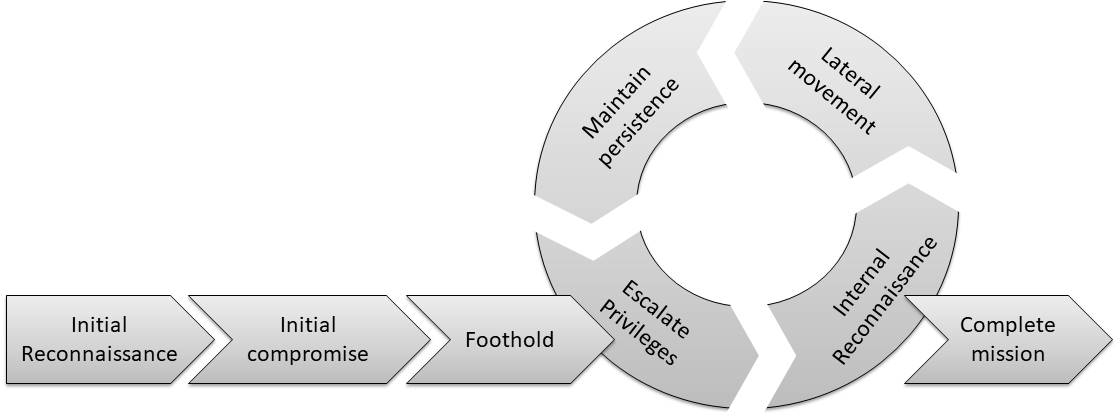
\includegraphics[width=0.7\textwidth]{./img/attack-lifecycle.jpg}
    \caption{Mandiant/FireEye Attack Lifecycle \cite{FireEye2018}}
    \label{fig:alcycle}
\end{figure}

By design the cyber attack kill-chain is developed from the defensive perspective to eliminate the adversarial threat and cyber attack at every stage of its execution. When considering the kill-chain from the attacker's perspective it is critical to be able to counter the kill-chain by applying novel \gls{tttp} to successfully execute every attack stage without being detected and disrupted. Therefore, cyber red team engaged in computer network operations have to employ adequate \gls{tttp} to raise the level of success.
The table \ref{tab:achain} on page \pageref{tab:achain} attempts to represent the stages of every individual approach, and groups them to create the cyber attack kill-chain with the most important stages of the attack, to give enough detail to the initial attack, internal lateral movement, and asset reconnaissance stages. In the table, the \textit{`X'} denotes, that a particular technique is directly applicable for countering a particular stage of the cyber attack kill-chain, and \textit{`S'} identifies, that this method can be used to support countering that particular stage in combination with other applicable approaches and tools.
The cyber attack kill-chain stages are mapped against the methods and techniques presented in the publications, which are applicable to countering or mitigating the effects of every cyber  attack kill-chain stage. This allows the \gls{crt} to adapt and assess their \gls{ttp} applicability to allow the \gls{cno} execution with a higher success rate.

\begin{figure}[!htb]
    \centering
    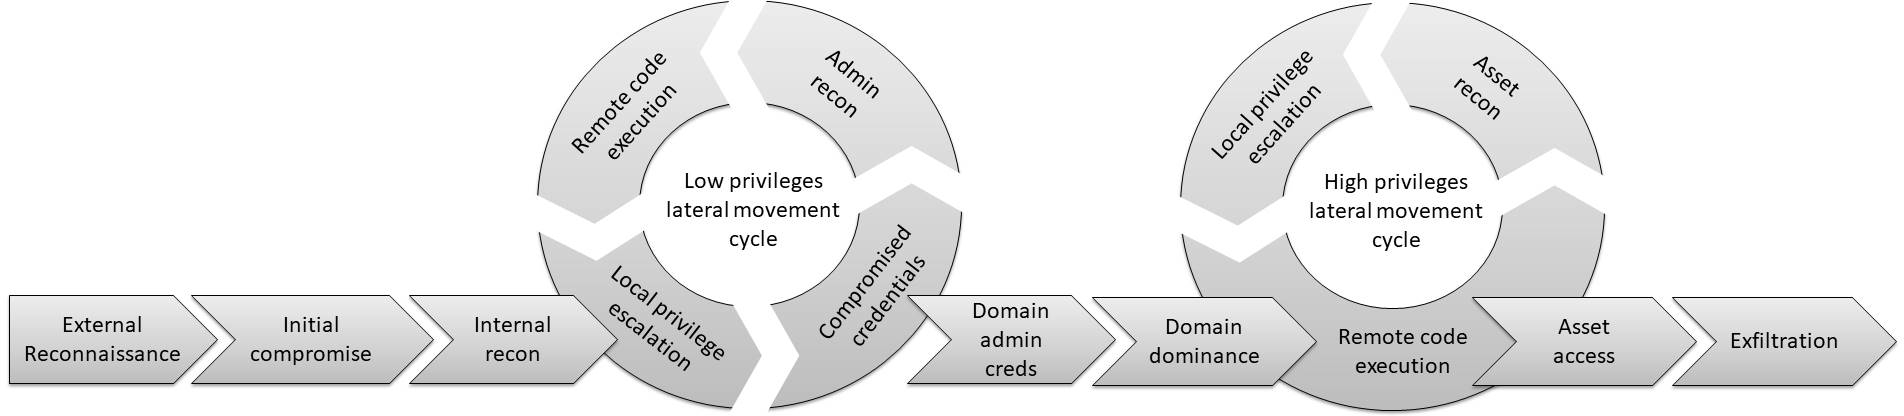
\includegraphics[width=1.0\textwidth]{./img/attack-kill-chain.jpg}
    \caption{Microsoft Attack Kill Chain \cite{Microsoft2018}}
    \label{fig:akchain}
\end{figure}

To address the strengths, weaknesses, and synergies of the popular cyber kill-chains, the author proposes an unified cyber attack kill-chain approach (Table \ref{tab:achain} on page \pageref{tab:achain}, column ``Cyber Attack Kill Chain''). The proposed model (Fig. \ref{fig:cakchain}) consists of the following phases: reconnaissance, initial compromise and foothold, command and control, internal reconnaissance, lateral movement, privilege escalation, persistence, asset reconnaissance, and objective completion. In this model, the reconnaissance and persistence loops are intertwined, with internal reconnaissance permitting lateral movement, privilege escalation and persistence, and allowing to conduct further reconnaissance activities on intended targets. If any applicable information or vulnerability is identified within the reconnaissance and lateral movement phases, the privilege escalation and persistence can be performed if necessary. However, not always privilege escalation and persistence are required to achieve the designated effect, therefore objective can be accomplished as soon as the intended target is located and the adequate network position and level of privileges have been obtained to perform the assigned task.

\begin{figure}[!htb]
    \centering
    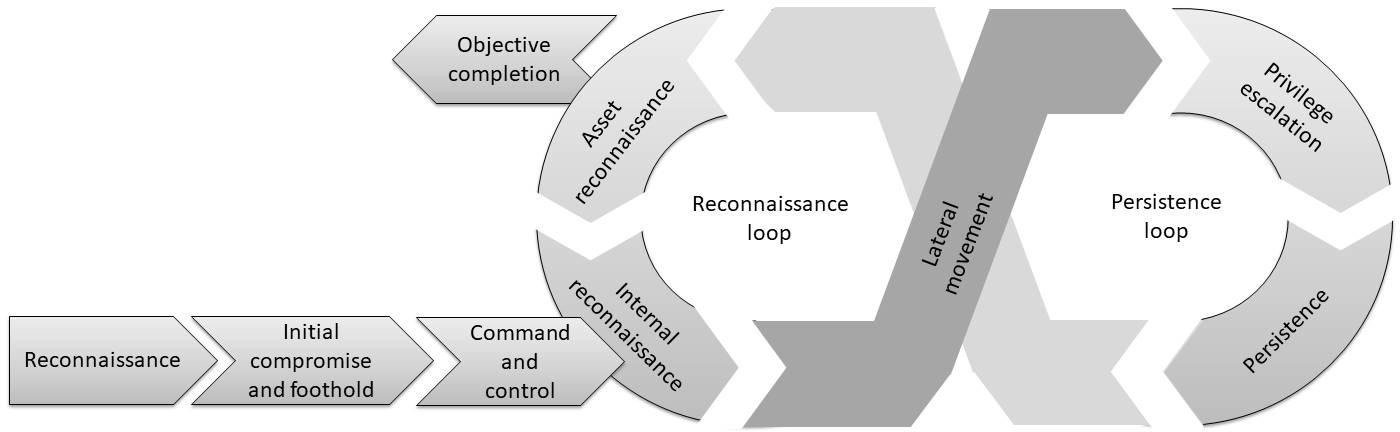
\includegraphics[width=1.0\textwidth]{./img/cyber-attack-kill-chain.jpg}
    \caption{Proposed cyber attack kill-chain model}
    \label{fig:cakchain}
\end{figure}

As stated in the chapter \ref{sec:scrtop}, such specialized cyber red team responsive operations should be capable of delivering the maximum possible effect. With this in mind, the red team needs to ensure highest success rate at every performed stage matching the cyber attack kill-chain. Such procedures would allow the applicable technique and tool proper use for accomplishing the mission objectives, maintaining the \gls{opsec}, and own asset protection.


\subsection{Chapter Conclusions}
The table \ref{tab:scrt} on page \pageref{tab:scrt} shows that the proposed methods and techniques in the research papers, are applicable to the specialized \gls{crt} responsive \gls{cno} and cover all of the aspects of such operational \gls{tttp} and demands. The majority of the proposed methods support the custom technique and tool development aimed at specific elements of the targeted system. This, with according tactics and procedures, results in a higher stealth level since these attacks are tailored to the intended objective to deliver the desired operational effects with highest impact possible. Additionally, these techniques are aimed at high stealth to provide a higher operational success rate, such as, establishing \gls{cnc} channel to circumvent the \gls{nids}. The tables \ref{tab:fuzz} and \ref{tab:tun} compare the author's developed methods against the other popular solutions. These unique and bespoke techniques are more effective when compared to relevant and commonly used ones (\ref{pub:firstPub}), grant the ease and flexibility to increase the speed of operation execution (\ref{pub:secondPub}), and allow focus of force on the most critical components of the target system (\ref{pub:thirdPub}). Based on the validated research in the publications, there are no other identified known approaches publicly available to match the level of the developed and presented techniques and tools. All of the proposed new techniques in this chapter have been implemented into the cyber red team oriented technical exercise series ``Crossed Swords'' and is described in a more detail in the chapter \ref{sec:exercises}.

A new unified cyber attack kill-chain method is introduced (Fig. \ref{fig:cakchain}) to find the synergies among the accepted kill-chain models to mitigate the gaps and emphasize their strengths.
The methods and approaches, proposed in the publications, are aimed at producing the desired effect and objective completion in the final stages of the cyber attack kill-chain. As it is identified, they cover all of the kill-chain stages either directly or can be used to support countering most of the stages, such as, allowing a local privilege escalation exploit delivery to the target system over the established covert \gls{cnc} channel.
The ultimate goal for the presented techniques is to grant the most benefit to the \gls{crt} from both the operation execution and objective accomplishment. When comparing their applicability both to specialized \gls{crt} responsive \gls{cno} execution and countering the cyber attack kill-chain, it can be assessed, that they provide a balanced approach and support to achieving the presented demands.


% Further chapters
\section{ADVERSARY DETECTION AND RED TEAM ASSET PROTECTION}
\label{sec:protection}
\glsresetall
The cyber red team has to maintain the visibility over the defended infrastructure and its own assets to ensure tracking of malicious activities, perform adversary assessment, gather further technical information aiding the attack trace-back and attribution, and protection of red team's operational infrastructure. Such detection and asset protection techniques benefit the cyber red team responsive operation execution and from the \gls{ooda} loop perspective they contribute to the observation and orientation actions.
Additionally, \gls{opsec} requirements have to be complied with to protect cyber red team assets, which are composed not only from the hardware and deployed software entities in cyberspace, but also the team identity and their operational goals.
Applicable techniques and solutions are presented in the listed publications (\ref{pub:fourthPub}, \ref{pub:fifthPub}, and \ref{pub:sixthPub}) and suitable use cases are assessed.

In contrast to a widely accepted belief, that attack is the best defence, the attackers might forget about defending their own assets and fail at insuring appropriate operational security measures. Such mistake can jeopardize the whole operation and lead to the full compromise of the cyber red team's infrastructure. This, most importantly, comes into consideration when the adversary is not only engaged in attacking the target infrastructure, but might pursue the defenders engaged in a responsive cyber defence. It has to be assumed that for every action there could be a counter action performed, thus leading to counter-red team operations and even to counter-counter-red team operations.
Defending party, executing a responsive cyber operation, is conducting operations from the infrastructure outside their defended network, which requires an equal and, in most cases, better protection. Such requirements stem from not only the threat detection perspective, but own asset, position, sensitivity of the pursued operational goals, infrastructure and identity protection requirements.

To provide such capabilities, the cyber red team has to have the expertise to implement, configure, supervise and monitor the threat detection solutions.
Such defence has to be implemented to cover the red team infrastructure's perimeter, as well as, activities happening within.
For the execution of crucial cyber operations the required red team environment would be custom made and deployed according to the operational needs, and afterwards securely destroyed.
To ensure such demands, the implemented defensive solutions have to meet at least the following criteria: readily-available, ease of deployment and management, flexible and scalable, high level of automation, and lightweight. Additionally, such solutions should be easily integrated with the technologies already present in the deployed network infrastructure elements, such as, \textit{rsyslog} or \textit{Syslog-ng} system logging services. Furthermore, these techniques, as well as the rest of the infrastructure, should be maintained to be as untraceable as possible and complicating the attribution. For such matters well developed, readily-available, non-commercial or open-source solutions providing high customization and flexibility would be applicable.
Two approaches complying with these requirements have been identified as system log (i.e., Syslog) based analysis and cyber deceptions.

In addition to automated syslog-based detection and cyber deception techniques, other threat assessment solutions can be used as well. Such solutions should comply with the mentioned criteria to be applicable for the cyber red teaming requirements. The proposed framework, named \textit{TED} (\ref{pub:ninthPub}), can be used on any modern GNU/Linux system with operating-system-level virtualization solution \textit{Docker} deployed. Foremost, such approach would be primarily used in the first stages of incident response on the systems, where no acceptable level of protection and threat detection solutions have been deployed or requiring additional in-depth assessment. \textit{TED} bundles most common local system and \textit{ELF} binary file security assessment tools, such as, \textit{checksec.sh}, \textit{Lynis}, and \textit{Spectre/Meltdown} checkers. All of the tools, their dependencies, management and orchestration scripts are included in a \textit{Docker} container, which can be used either in Internet connected or disconnected systems, and requiring only single requirement of \textit{Docker} engine being present. This engine is included in majority of the popular modern GNU/Linux distribution repositories and, in most cases, already being installed on systems, such as, application, and web servers. Such lightweight solution allows it to be easily used to establish system security level and identify potential binary file attacks, without introducing significant changes or requirement of installing other solutions on the target system, thus minimizing the contamination of the examined system. The potentially compromised system analysis has to be performed according to the digital forensics requirements, with assessing the system compromise likelihood and at least acquiring memory and disk images, before proceeding with more intrusive activities. Such activities may provide the needed situational awareness picture and assist initial technical attribution establishment, before engaging the specialized cyber red team into the computer network operations against a suspected actor in the cyberspace. Whenever the cyber red team moves from their defended information system into their operational infrastructure, from where the responsive operation will be carried out, the deployed assets in that infrastructure, in most cases, become disposable if deemed compromised. \textit{TED} may be used to assess the required hardening level of the initially deployed operational systems or in specific cases -- to examine the cause of their compromise. The primary solutions, compliant with the requirements and to be used within the defended and operational infrastructures, consist of system log file-based anomaly detection and cyber deception solutions.


\subsection{System Log File-Based Anomaly Detection}
System log file monitoring and analysis has been acknowledged as an important network and system management technique, as well as, granting the possibility of detecting anomalies and security violations.
Under normal circumstances, all network devices, such as, hosts, sensors, networking equipment or sophisticated data parsing and threat detection solutions, should be able to generate alerts and system logs in a textual format. It is highly recommended for such data to be delivered to a centralized storage location for retention, further analysis and correlation. Depending on the solution, the generated alerts and system logs can have a different representation, which might be parsed either without additional processing or requiring normalization or transformation to an unified standard. Despite this, easy to deploy and flexible system log processing and correlation method implementation into the cyber red team tool-set could grant the required visibility over the defended and protected assets.

Such system log file analysis should be performed for the defended network infrastructure, as well as, the operational one used by the red team.
Despite both environments collecting the log files, their design implementations could differ. Defended infrastructure could generate and record events in the log files, which are then transferred to the central location for retention and analysis, depending on the security policies and other requirements. The protected cyber red team operational infrastructure would follow similar approach, however, it might be beneficial not to keep the log files on the red team hosts or its supporting infrastructure, but directly delivered to the central secure location for immediate analysis and threat assessment. Such approach would be considered in case of a likely counter red team operation execution by the adversary and attacker possibly gaining access to the defending red team's infrastructure elements. This potentially could minimize the exposure regarding the executed responsive activities, intended goals and attribution.

Event correlation has established itself as a prominent and recognized monitoring technique, which is essential for establishing situational awareness.
The Simple Event Correlator (SEC) (\ref{pub:fourthPub}), written in Perl, runs on all modern UNIX based platforms, has been used for a wide range of purposes and environments as an efficient open-source alternative to the commercial solutions. This solution is designed for real-time event processing and incorporates event matching, parsing, and output generation.
The SEC uses scalable rules for event correlation, which can be applied to a range of inputs, including the Syslog files.

This lightweight, flexible and real-time nature of SEC complements the cyber red team operational requirements, allowing focus on the operation itself while gathering and receiving real-time alerts. Such visibility, enhanced by the user interface such as \textit{Kibana} from the \textit{ELK Stack}, can deliver the required situational awareness regarding the cyber red team's operational infrastructure. Gained awareness not only allows pinpointing the system failures or monitor the infrastructure performance, but allows to detect anomalies, such as, attacks or unsanctioned access attempts.

Despite the SEC being powerful event correlation solution, it relies on its rule-sets, which have to be created by the human analyst.
A novel data mining-based framework is developed (\ref{pub:fifthPub}), requiring no human intervention, for fully automated rule discovery for real-time detection of anomalous messages from Syslog-based logs. This approach possesses the capability to adapt to the changes in the system and employs the \textit{LogCluster} algorithm for data mining.
Human expert can extend the framework with own created rules, thus aiding the anomaly detection or adjusting the system to the specific design implementation or operational goals.

The detection of previously unknown error conditions and anomalies has been a difficult problem, however, the proposed framework provides a one practically applicable solution to it. The cyber red team implementing this solution on the centralized Syslog collector, to which the individual host system logs are transferred over a reliable and encrypted channel, gains an immediate benefit with least efforts required.
As the conducted experiments over a larger period of time have indicated, the anomalies and unexpected system state conditions have been successfully identified. Furthermore, the test involving the running of \textit{Bbuzz} fuzzing framework for abnormal network communication generation, clearly confirms that unknown anomalous or malicious requests, resulting in the Syslog entries, are detected and reported.
It has to be noted, that cyber red team protected operational infrastructure should implement also the traditional defensive mechanisms (i.e., passive defence), such as, packet filtering on all network hosts (e.g., \textit{iptables}, \textit{ip6tables}, \textit{Firewall \& network protection}), deploy proper system hardening (e.g., \textit{SeLinux}, application white-listing), host protection with \gls{hids}, system disk encryption (e.g., \textit{LUKS}, \textit{BitLocker}, \textit{VeraCrypt}), and user privilege level separation and control. When deploying the defensive measures, they have to be assessed from the operational security considerations to confirm, that no information is leaked out from the infrastructure to the third parties, such as, anti-virus, \gls{hids} or \gls{ids} alerts and metrics.
When considering a potential counter-red team operation executed by an adversary the similar attack approaches have to be expected and system protection should be augmented by the out-of-band (e.g., hardware or software-based port mirroring) network traffic monitoring and analysis solutions, such as, \textit{Snort}, \textit{Suricata} and depending on available resources and team capabilities -- \textit{Bro} and \textit{Moloch}. These solutions in turn would also generate the alerts and system logs, which can be transferred to the central location for the data mining, correlation and security incident information extraction.
If the cyber red team assumes the high risk of the counter-red team operation plausibility, then further in-depth system monitoring solutions can be considered for deployment to deliver additional visibility, such as, system performance metrics (e.g., \textit{sysdig}, \textit{Telegraf}), kernel requests (e.g., \textit{Snoopy}), unsanctioned system use (e.g., \textit{tripwire}).


\subsection{Cyber Deception-Based Detection}
All of the presented passive monitoring and threat detection techniques should be augmented with the active cyber defence elements within the cyber red team's operational infrastructure.
The most prominent one, as described in the chapter \ref{sec:rcd-work}, has been identified as the cyber deception approach.
If deployed either in the defended system or in the protected cyber red team operational network this set of techniques would grant the immediate feedback to the cyber red team on any identified suspicious activities.
Cyber deceptions can further be integrated to deliver their system logs and alerts to the central Syslog processing location.
Various types of cyber deceptions can provide different levels of adversary tracking and technical attribution information gathering. The solutions, such as honeypots, would be able to identify unsanctioned access to them and collect information on adversary's activities within the decoy network allowing a better insight into their capabilities, intentions and \gls{tttp}.
Honeytokens could potentially allow the trace-back to the location from where such data has been executed or accessed.

The following cyber deception frameworks were implemented in the reference network, against which the targeted attacks were launched (\ref{pub:sixthPub}) -- \textit{T-pot}\footnote{DTAG Community Honeypot Project. \url{http://dtag-dev-sec.github.io/}. Accessed: 05/10/2018}, SHIVA\footnote{Spam Honeypot with Intelligent Virtual Analyzer. \url{https://github.com/shiva-spampot/shiva}. Accessed: 05/10/2018}, YALIH\footnote{Yet Another Low Interaction Honeyclient. \url{https://github.com/Masood-M/yalih}. Accessed: 05/10/2018}, KFsensor\footnote{Advanced Windows Honeypot System. \url{http://www.keyfocus.net/kfsensor/}. Accessed: 05/10/2018}, and ADHD (see footnote \ref{fnote:adhd} on page \pageref{fnote:adhd}).
To conduct the experiments the target network consisted of various zones, such as, demilitarized network hosting external web and e-mail services, internal network for business purposes hosting MS Windows and GNU/Linux clients, and a sub-net for information system security monitoring solutions. Every sub-net represents location for deployment of an applicable cyber kill-chain technique both from the attacker and the defender perspectives. The cyber deceptions, according to their applicability and expected use cases were deployed in the network segments to match the defender's requirements on stopping the attack according to the cyber attack kill-chain stages.
Every particular framework or a collection of tools is either oriented towards being deployed on its own client operating system (e.g., GNU/Linux, MS Windows), is a high- or low-interaction honeypot oriented at deceiving the adversary or is a set of tools to be used to actively detect, counter or degrade the attacker's capabilities (e.g., port-spoofing, \textit{tarpit}). The experiment results identified, that out of all implemented technologies the multi-honeypot platform \textit{T-pot} proved to be the most efficient in identifying and detecting attack or malicious activities. \textit{T-pot} includes a set of \textit{dockerized} instances of multiple solutions, such as, \textit{Glastopf, Kippo, Honeytrap, and Dionaea} honeypots, \textit{Suricata} \gls{nids}, \textit{ELK} stack, and \textit{ewsposter} for honeypot data sharing.
The cyber deception is a valid method for detecting, deceiving, disrupting, degrading, denying, and defending against the adversary.

\textit{Detect}. As this being one of the core requirements for any defensive activity, it is required to establish the situational awareness and allow pursuing responsive activities against the detected threat. All of the mentioned passive methods and further described active ones, contribute to achieving this goal. To complement attribution via the active detection means, the most prominent approach could be various cyber deception techniques, such as, \textit{honeytoken} documents rigged with an executable code, or strategically placed decoy data leading the attacker to the deployed honeypots. Rigged documents, such as, attack orders, technical documentation, or other sensitive information, once exfiltrated from the defended infrastructure and opened by an attacker potentially could reveal the adversary position in the cyberspace by \textit{beaconing} its IP address and other sensitive data collected and sent by the embedded computer code. Depending on the adversary's operational security methods, such as, rigged files might be either stripped of executable scripts, opened on an isolated or third-party system, or modified to deliver false information. Despite these concerns, this option should be practised by the cyber red team to raise the level of attribution in case the cyber deceptions are well crafted and placed or if the adversary is careless and makes a mistake.

\textit{Deceive}. Part of defensive activities, especially ones implemented in the cyber red team's operational infrastructure, should be aimed at confusing and deceiving the adversary by any means possible. The techniques, such as, decoys and cyber deceptions will not only allow the identification and tracking of the adversary, but would also allow its attribution, technical capability and goal assessment. The concept of cyber deceptions would include solutions, such as, honeypots which would spoof the attack surface by deploying large quantities of simulated hosts or network topologies (i.e., honeynets). Besides providing deception this technique also supports the degradation of attacker capacity, since adversary would be entangled in sorting identified systems between the real and fake ones. Both low- and high-interaction honeypots benefit the attribution process, additionally granting the insight into adversarial \gls{tttp} in case of a high-interaction honeypot usage. It has to be noted, that high-interaction honeypots might require a larger effort for maintenance and upkeep in contrast to the low-interaction ones but would also give a better understanding of the adversarial objectives and motivation. However, it would be highly suggested to have at least the low-interaction honeypots embedded in the red team's infrastructure.
To further control and deceive an adversary decoys could be placed throughout the red team's operational infrastructure. The strategically placed decoys (sometimes called ``breadcrumbs''), for example, in the form of cached credentials, saved remote connection sessions or mapped network drives, would try to force the attacker use this seemingly valuable information to follow the predefined path designed by the defender leading to a decoy system. Once this decoy information is used against the decoy system (e.g., honeypot), the alert is triggered, and further perpetrator actions can be monitored and traced. One of the rising solutions in providing such cyber decoy systems based on sophisticated scenario development, ``breadcrumb'' creation and placement is the \textit{Mazerunner} (see footnote \ref{fnote:mazerunner} on page \pageref{fnote:mazerunner}).

\textit{Disrupt}. If a detected and identified attack becomes too intrusive or tries to overwhelm the protected infrastructure, it is possible to disrupt the connections either by firewalling or \textit{null-routing} them. Such action does not directly aid the attribution or adversary assessment, however, can be used to indirectly limit available attack paths thus potentially steering the perpetrators towards the desired communication channels or approaches which can be controlled or monitored by the cyber red team. Depending on the situation, it might be chosen not to disrupt the adversary activities within the protected networks, but to carry on observing and analysing them to gain more intelligence information on the threat actor.

\textit{Degrade}. Any active or responsive action depends on time, thus deception and degradation approaches are used for the defenders to gain additional time to respond while opponent is being tricked in performing useless activities. Degradation by inflicting the time penalty is typically executed by at least the following approaches -- honeypots to artificially increase the network complexity and size for the attacker to spend time on probing it, network host attack surface spoofing to force attacker wasting time on performing endless network port scans, and \textit{tarpitting} incurring a serious time cost when dealing with slowly responding services to all requests. In some cases, degradation would be seen as better approach instead of disrupting, due to the fact that the adversary will still attempt to invest time instead of leaving or searching alternatives.
In cases when active engagement against enemy communication channels or capabilities is executed, the opponent will comprehend that they are being deceived or caught and might change their tactics and approaches. Depending on the situation this might be desirable to observe the true potential and capacity of the threat actor.

\textit{Deny}. If disrupt and degrade are active engagements against already ongoing attack and its paths, the denial would proactively assess and anticipate attacker's goals and eliminate the attack paths even before they are pursued. This could be linked together with detection and deception techniques, where adversary presence and goals are identified and isolated to limit their movement within the defended network. For such option to be feasible, all of the infrastructure hosts should be centrally manageable through the solution, such as, \textit{Salt} stack. However, if such central management solution is taken over by the adversary then the cyber red team could potentially lose all their assets and the operation becoming fully compromised.

\textit{Defend}. The overarching concept merging all of the individual approaches to provide the unified goal for guarding either the defended information systems or protecting the red team's assets and operational infrastructure.


\subsection{Cyber Red Team Operational Infrastructure Protection Considerations}
\label{sec:opinfra}
The proposed conceptual model for cyber red team's operational infrastructure (Fig. \ref{fig:rtinfra}) consists of multiple logical network zones, designated by their purpose and usage. This comprehensive infrastructure model is just one of the possible variations, and will be dependant on the operational requirements, resources and time available. The figure represents the infrastructure concept design, functional area purpose and host description, and deployed defensive measure applicability. The key factor in this operational network prototype is to assess which of the described and researched techniques and tools for the detection and deception are applicable and in what ways.
This cyber red team operational infrastructure model has been implemented to a certain extent in the technical cyber exercise ``Crossed Swords'' and is covered in more details in chapter \ref{sec:xs}.

From the previously assessed approaches on Syslog-based anomaly and cyber deception based detection, the following techniques are considered: 
\begin{enumerate}
    \item \textit{passive defence}, supporting defend, disrupt, and deny activities, focuses on host and network device hardening, packet filtering, \gls{nids}, communication channel redundancy, security and encryption, and network segmentation;
    \item \textit{Syslog analysis}, supporting detect activity, aims at anomaly and threat detection by analysing aggregated system log and alert information from the network nodes;
    \item \textit{Attack surface spoofing}, supporting degrade and deceive activities, is a form of cyber deception for spoofing a large attack surface to confuse and stall the adversary;
    \item \textit{honeypot}, supporting deceive, degrade, and detect activities, is a form of active threat detection and can be used for adversary activity tracking, attack surface spoofing (e.g., honeynets) and stalling the movement of attacker within the network;
    \item \textit{cyber decoy}, supporting deceive, degrade, and detect activities, is a form of a decoy, such as, the ``honeytoken'' or ``breadcrumb'' information deployed on network hosts, to lure the adversary towards a detection system (e.g., honeypot) or to reveal its current position in the cyberspace (e.g., beaconing); and
    \item \textit{tarpit}, supporting degrade activity, directly aims at stalling the incoming attack progression by responding slowly to received requests.
\end{enumerate}

\begin{figure}[!htb]
    \centering
    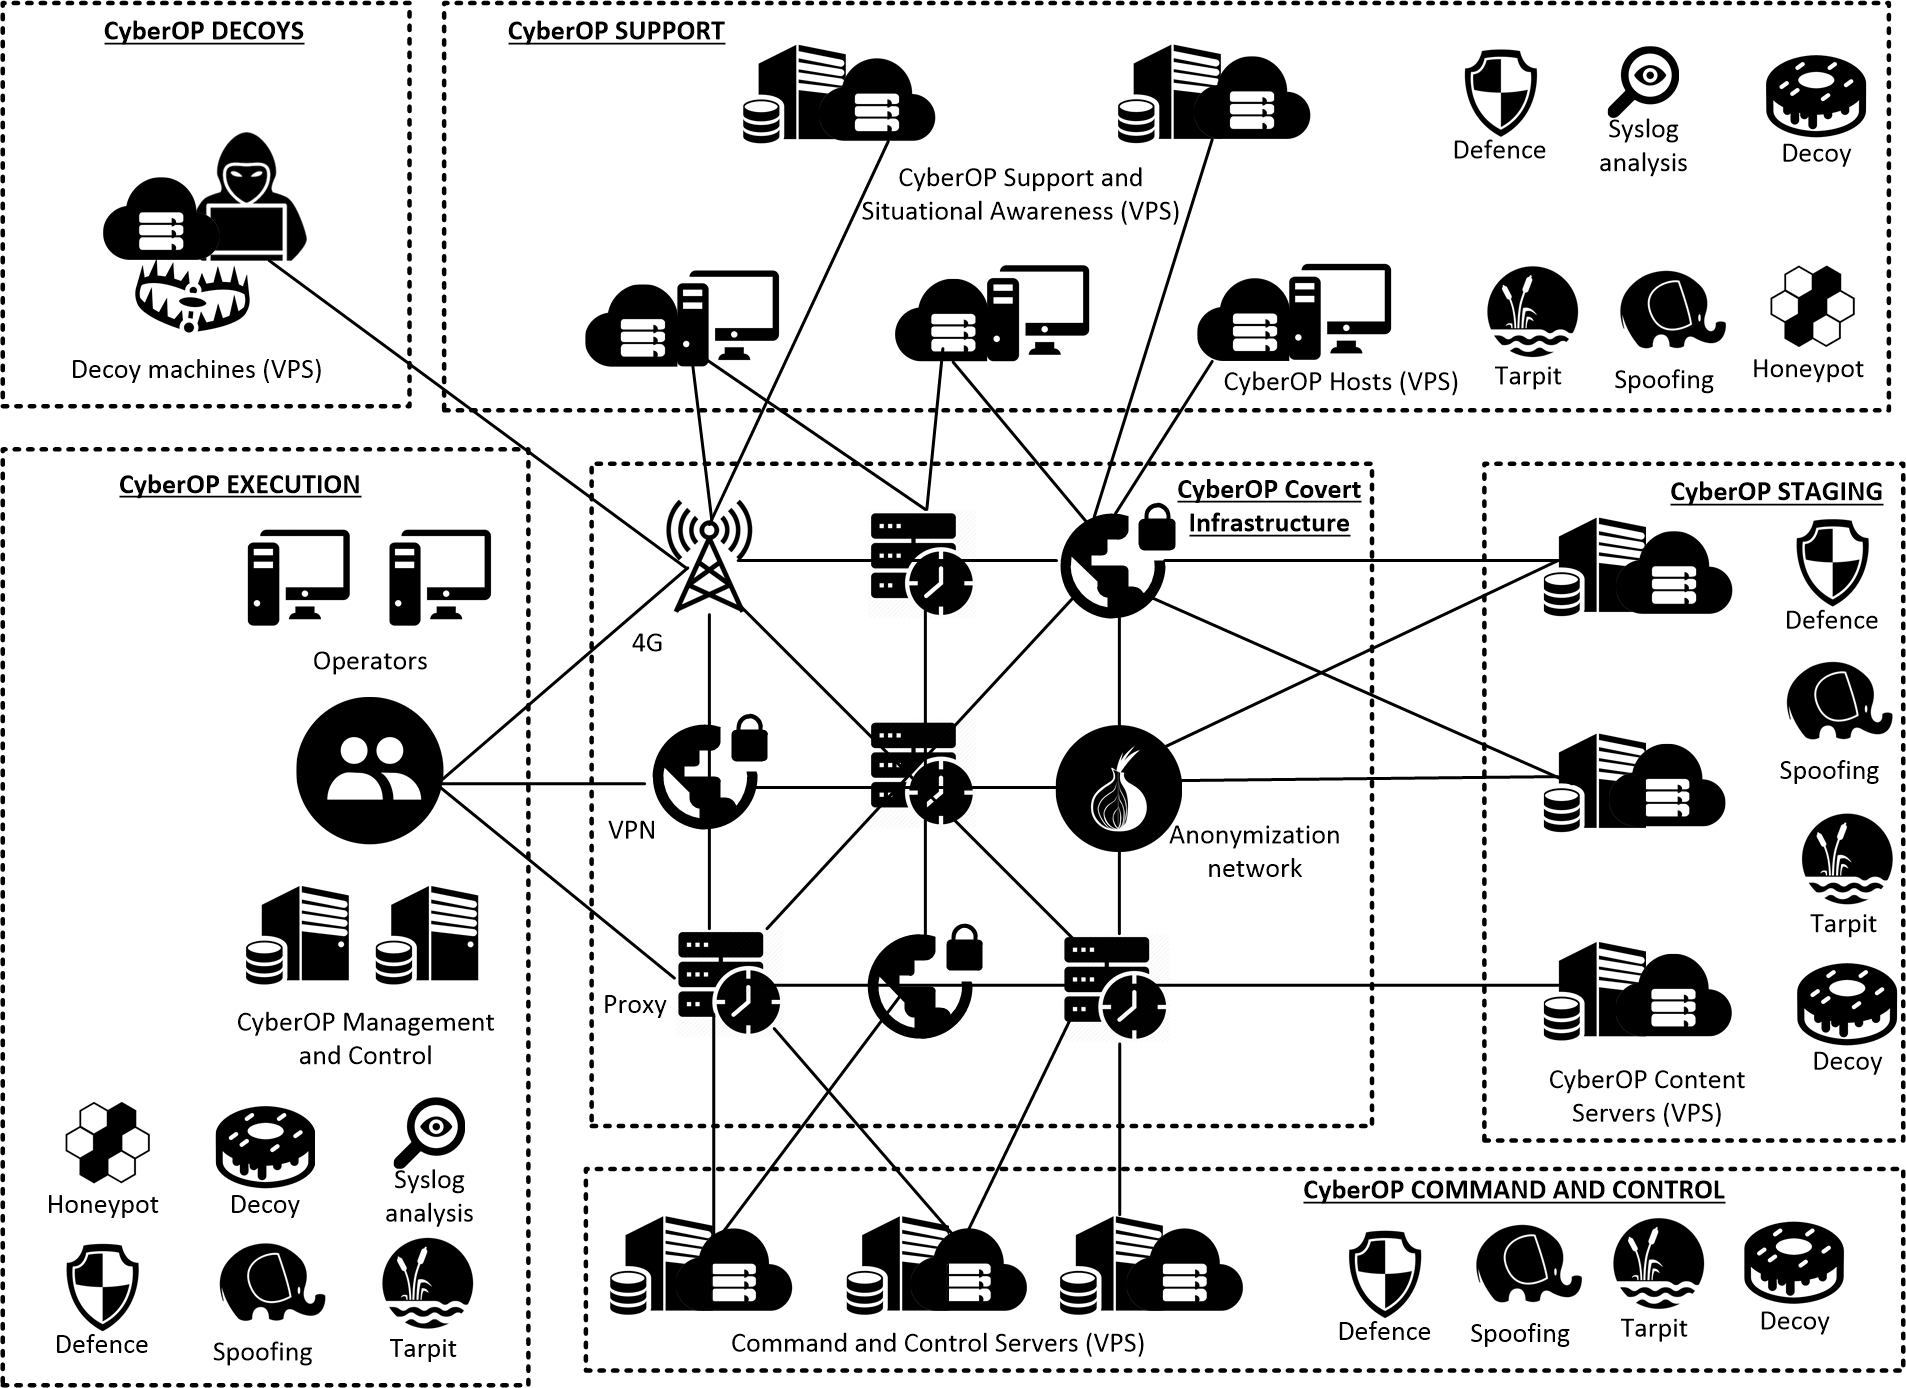
\includegraphics[width=1.0\textwidth]{./img/crt_infra.jpg}
    \caption{Cyber red team operational infrastructure concept model and defence measures}
    \label{fig:rtinfra}
\end{figure}

Cyber operation covert infrastructure is a set of interconnected nodes on the Internet by the use of various communication technologies, such as, mobile 4G data connections, VPN tunnels, proxy servers, connection bouncers, or anonymization networks (e.g., TOR, i2p). The purpose of the covert infrastructure is to ensure the maximum possible un-traceability to the origin of the cyber red team operators connecting to their deployed assets in the cyberspace. Depending on the operational requirements, at least two network hops should be taken. Relying upon the design of such covert network, the interconnections between the nodes can be changed dynamically whilst maintaining and ensuring the overall connectivity between the two or more interconnected nodes or groups of nodes engaged in the cyber red team operation.
Various design approaches can be chosen and implemented to design the overall cyber red team infrastructure and divide it in logical groups basing on their purpose and usage. This might depend on various factors, such as, if a particular adversary \gls{tttp} are impersonated for the ``false-flag'' operations, complexity and sensitivity of the performed computer network operations, available resources, and if the cyber red team wants to expose the advanced capacities and capabilities it possesses. For example, a covert network for a high value computer network operation aiming at executing a sophisticated targeted attack against adversary information systems and establishing a \gls{cnc} control over the compromised nodes, might have the following architecture requiring applicable defensive measures (Fig. \ref{fig:rtinfra}):
\begin{enumerate}
    \item Cyber operation execution area, where the cyber red team is located and the connections to their assets in cyberspace over the covert infrastructure is established. This \textit{home} network would host not only the computer systems from which the operation is originating, but also supporting systems, such as, the situational awareness provision, operation tasking and organisation, collected information cataloguing, indexing and management, operational network supervision, testing, research and development systems, and covert infrastructure automated creation, administration, adaptation and destruction.
    In this area all of the protection techniques, passive defence, Syslog analysis, spoofing, honeypots, cyber decoys, and tarpits, are applicable to provide maximum possible defence for the cyber operation origin and execution orchestration;
    \item Cyber operation support area, where hosts engaged in conducting and supporting the computer network operation are located. All of the nodes are automatically deployed, hosted and afterwards securely destroyed (e.g., overwriting the encrypted file system with random data, such as \textit{/dev/urandom}) on a purchased \gls{vps} operator infrastructure. These nodes are supported by the deployed \gls{vps} systems, such as, operational infrastructure supervision, Syslog aggregation and analysis, and secured immediate operational information storage.
    The same protection mechanisms as for the cyber operation execution area are applicable here as it is a vital set of assets on which the success of the operation depends;
    \item Cyber operation staging area hosts the exposed \gls{vps} nodes engaged in delivering or hosting the attack artefacts. This would include systems, such as, SMTP servers for sending e-mails to the target, web servers for hosting the malware and dive-by exploitation kits, and target network reconnaissance tools. These hosts are used for direct interaction with the adversary for activities, such as, reconnaissance or initial foothold establishment. Taking into account that these systems, due to the nature of their usage, can be identified by the target, a pool of active and stand-by systems are required to be changed once they have been discovered or have fulfilled their intended purpose.
    Furthermore, this area can include not only the assets deployed by the cyber red team on the public \gls{vps}, but also any other public or cloud-based solutions, for example, \textit{Dropbox} for hosting malicious payloads, \textit{Google docs} end for credential harvesting, and \textit{Twitter} feed for \gls{cnc} command issue. Such public service utilization raises the level of scalability, set-up and destruction, minimizes the expenses and time investment, as well as benefits to raising the level of anonymity.
    This group of assets due to their high exposure nature and direct engagement with the target have to possess a set of protection mechanisms allowing to estimate asset compromise and tracking of adversarial activities. The techniques, such as, passive defence, spoofing, tarpitting, and decoys, are applicable to ensure a decent level of protection, however, without having a straightforward link, even using covert infrastructure, back to the cyber operation support area. Instead decoys would try to lure the attacker towards the cyber decoy area \gls{vps} hosts instead, which then would report any detected activities back to the cyber support area servers. Varied choice for protection technique tools and implementations should be employed across all protected assets to limit the cyber infrastructure host fingerprinting and identification within the cyberspace based on the defensive and techniques in use;
    \item Cyber operation command and control area is the set of \gls{vps} based nodes hosting the \gls{cnc} \gls{vps} servers. Upon a successful attack from the cyber operation staging area, the compromised hosts are designed to call back to the intended \gls{cnc} servers. The connection to the \gls{cnc} servers is handled via the redirectors in the cover infrastructure, thus limiting the direct exposure of this critical asset. However, the possibility of their detection and targeting by the adversary exists, therefore a set of active and hot stand-by \gls{cnc} servers is required to transfer the control from one to another in case one has been identified or compromised.
    Exactly the same protection considerations are applicable to this area as for cyber operation staging hosts due to the high exposure and direct interaction with the target information systems; and
    \item Cyber operation decoy area is the landing area to where the stored decoys would attempt to lure the adversary, which is trying to take control over the cyber red team assets and tracing back to the origin of attack. This area would host nodes, such as, honeypots, and sensors for \textit{honeytoken} beacons. The detected interactions with these decoys would be logged and sent to the cyber operation support area servers, such as, Syslog collection and analysis.
    In this area, systems, such as, the honeypots, decoy destination, and beaconing detectors, are deployed. Since these hosts are designed for actual interaction with the adversary, it would be advisable for them to be designed to look as legitimate as possible to make the attacker believe that some actual cyber red team operational hosts have been reached and thus reveal their position and \gls{tttp}. However, still having some level of hardening implemented to deny full compromise of the hosts. Depending on the cyber operation infrastructure goals, the high- and low-interaction honeypots or a mix of both could be implemented, taking into consideration, that high-interaction systems, in comparison to low-interaction ones, would deliver a more believable experience, but demand higher maintenance and can be potentially fully compromised. Adaptive self-configurable honeypots \cite{Wagener2011} \cite{Zhang2017} allowing the adjustment to the incoming attack to provide the highest possible level of interaction and experience for tracking the adversary and permitting to perform threat assessment.
\end{enumerate}
Author acknowledges that \gls{ai} technologies, such as, artificial neural networks and machine learning, should be considered for cyber red team operational network design, implementation and protection.
Also, the MITRE ATT\&CK and PRE-ATT\&CK \cite{MITRE-ATTACK} can be considered for cyber red team \gls{opsec} requirements and when being engaged in false-flag operations with particular threat actor's \gls{tttp}.
Furthermore, the protection has to be ensured for cyber red team obtained and controlled assets, such as, DNS names, virtual private servers, bullet-proof hosting services, social network profiles, \gls{osint} tools (e.g., Shodan, Maltego, VirusTotal \gls{api}), cloud services (e.g., MS Office 365) and payment methods. However, such protection mechanisms would more revolve around using privacy and anonymity ensuring services, use of covert infrastructure for their access, have unique accounts and associated registration data, payments by hard to trace methods (e.g., crypto-currency, )

\subsection{Chapter Conclusions}
This chapter examines the use and applicability of the detection and deception solutions for integration into the cyber red team life-cycle and asset protection. The described novel log-based anomaly detection approaches (\ref{pub:fourthPub}, \ref{pub:fifthPub}) and existing cyber deception solutions (\ref{pub:sixthPub}) deliver the required effects to benefit the \gls{crt} conducted operations, such as, adversary tracking, threat assessment, technical attribution, red team asset protection, \gls{opsec} improvements, and situational awareness. While conducting the responsive computer network operations the \gls{crt} has to bear in mind, that the pursued adversary might engage in the counter-red team activities, thus endangering the not protected \gls{crt} assets and jeopardizing the whole responsive operation. Additionally, solutions, compliant with cyber red team operational requirements, can be used for initial response to confirm the defended system security breach and gather initial technical attribution information (\ref{pub:ninthPub}).
The proposed concept model for the cyber red team operational infrastructure (Fig. \ref{fig:rtinfra}) displays and explains the reasoning and benefits of the detection and deception methods deployed therein. Such model, if adapted and customized according to operational requirements, would provide the necessary situational awareness, increased stealth, and benefit to gaining advantage over the adversary.
\section{CYBER RED TEAM TRAINING}
\label{sec:exercises}
\glsresetall
Majority of the exercises are cyber defence oriented with the \gls{bt} being the primary training audience and the \gls{rt} role-playing the adversary to provide the learning experience for the defenders. However, technical exercises, oriented at advancing the readiness level and experience of a cyber red team, are lacking, limited in scope, not mentioned or described publicly. 
To enable the development of defensive approaches both approaches -- blue and red, have to be exercised, especially if they are dependent on each other both in technical exercises and in real-life operations for protected information system defence.
To integrate and explore the proposed concepts of \gls{rcd}, \gls{cno}, \gls{crt}, red team \gls{tttp}, detection mechanisms, cyber deceptions, and red team operational infrastructure, a unified environment is required. A technical cyber exercise oriented not only at training single facet of the cyber red team, such as, solving technical challenges, but implementing the presented components to create a cyber operation environment would increase the red team training experience. Additionally, cyber red team interactions and inter-dependencies with other operational entities, such as, conventional kinetic or special operations forces, should also be explored to see how cyber operations fit within the larger picture and not on its own.

This chapter, published in \ref{pub:tenthPub}, unifies all of the listed publications including \ref{pub:seventhPub}, with their respective contributions being implemented and assessed in the cyber red team oriented technical cyber exercise ``Crossed Swords'' created and the development being led by the author since year 2014. This exercise and its design considerations are represented as a use case analysis in this thesis.
The following sections, in a structured manner, introduce and explore the various aspects of the ``Crossed Swords'' exercise series as a case study, and emphasize the listed publication concept implementation and their assessment.

\subsection{Cyber Red Team Exercise Design}
\label{sec:xs}
Cyber exercise ``Crossed Swords'' (XS) \cite{XS18}, organized jointly by NATO CCD CoE and CERT.LV, is an annual international technical exercise oriented at training cyber red team with the latest technologies and striving to deliver high realism and training benefits. This exercise, created and with core technical aspects managed by the author, was initially introduced in year 2014 as a red team workshop aiming at training the allied cyber red teams and increasing their readiness for real-life operations. Since its inception, the exercise has grown in complexity and size with the development and management team consisting of over thirty renowned experts in the various areas of technology, red teaming, strategy and leadership, kinetic warfare, international law, and research. The exercise spans across three consecutive days representing a 24-hour fast-paced and intensive operation.
More importantly, this exercise has served as a platform for implementing, testing, confirming, and conducting studies in the areas of author's research. The proposed concepts, techniques, tools, and procedures as presented in the listed research papers have been applied and tested within this exercise.

To collect the feedback regarding the XS exercise, a survey was prepared and sent out to all former participants, with the purpose to establish a quick high-level overview.
The created survey, aimed at assessing the technological advancement, realism, complexity, learning benefits, and real-time feedback value, was created by the author and sent out to all participants since 2014. Out of 100 participants 33 have provided their feedback, which has been assembled and presented in appendix on page \pageref{app:survey}.
The survey asks to evaluate the following aspects of the exercise: level of realism of the executed cyber operations at the exercise, diversity of target systems implemented in the game network, technical challenge complexity level, exercise benefits and training outcome value, and the value of provided detected attack feedback. The respondents are requested to grade each of these categories in the scale from zero to five, where the 0 represents the very low realism, diversity, complexity, no value at all, and 5 -- very high realism, diversity, complexity, and extremely valuable.
The anonymous results gathered from the various alliance member nation participants, mainly representing military organizations, acknowledge the high realism of the exercise (graded 4 out of 5), high diversity of target systems (graded 4 out of 5), high complexity of technical challenges (graded 4 out of 5), with exercise training benefits being extremely valuable (graded 5 out of 5), and provided detected attack feedback being both extremely and very valuable (graded 4 and 5 out of 5). The grading values are a direct representation of the survey charts and are presented here with an illustrative purpose.


\subsection{Exercise Training and Mission Objectives}
\label{sec:to}
The exercise aims to address at least the following principles: 
\begin{enumerate}
    \item Cyber red team assembly and structure. Addresses how the cyber red team can be assembled and structured to accomplish the laid out operational tasks with as less management overhead as possible;
    \item Cyber operation execution. Explores how the assembled \gls{crt} performs and exposes the ability to accomplish the mission;
    \item Information and attack campaign management. Assesses the ways on how the \gls{crt} collaborates for information sharing and mission goal objective tasking;
    \item Red team coordination. Evaluates the \gls{crt} capability to coordinate the particular attacks to avoid tasking collisions, such as, interfering with other sub-team activities (i.e., ``friendly-fire'') or doing tasks already performed by other sub-team;
    \item Increased level of stealth. Ability of the \gls{crt} to apply proper \gls{tttp} to avoid detection at the best level possible;
    \item Technical sophistication and related \gls{tttp}. \gls{crt} capability to find innovative ways apply applicable \gls{tttp} to accomplish mission objectives;
    \item Fast-pace and time pressure. Explores how the \gls{crt} is able to perform under constant time pressure and conducts objective prioritization;
    \item Situational awareness. Looks at the possibilities to provide the situational awareness to the \gls{crt} to improve the learning benefits and outcomes;
    \item Cyber red team asset protection and \gls{opsec}. Identifies the applicability of \gls{opsec} requirements to increase the level of stealth, make attribution harder, and protect the \gls{crt} deployed assets;
    \item Adversary assessment, cyber intelligence and technical attribution. Inspects the \gls{crt} ability to gather information allowing adversary threat assessment and technical attribution;
    \item Target network infiltration and precision take-down. \gls{crt} capability for covert target network infiltration, asset identification and precision take-down;
    \item Legal ramifications of the cyber attack. Discovers the possible legal ramifications of the \gls{crt} performed activities and overall operation; and
    \item Cyber-kinetic interdependencies. Explores the ways on how cyber and kinetic operations can be integrated to assist each other within all applicable domains of operation.
\end{enumerate}
These principles are selected to represent and prototype of a full-spectrum cyber operation and to be used as a basis for the exercise development and execution.
Within this scope, the exercise is designed to implement the following cyber red team training objectives (TO):
\begin{enumerate}
    \item [TO1.] Perform defended system compromise assessment, practice evidence gathering and information analysis for technical attribution, identify the origins of malicious activities and take actions to stop them;
    \item [TO2.] Execute a responsive cyber defence scenario for adversarial information system infiltration;
    \item [TO3.] Employ stealthy attack approaches, and evaluate applicable \gls{tttp} for fast-paced covert operations;
    \item [TO4.] Exercise working as a united team in achieving the laid out mission objectives;
    \item [TO5.] Develop specialized cyber red teaming soft and technical skills needed for operation management, information flow, and target information system takeover; and
    \item [TO6.] Explore and evaluate the full-spectrum operation's cyber-kinetic interdependencies.
\end{enumerate}

Depending on the individual exercise over-arching scenario, the mission goals for the cyber red team might slightly vary, but the essential mission objectives (MO), which the red team has to accomplish are the following:
\begin{enumerate}
    \item [MO1.] Maintain situational awareness, ensure resiliency of the defended systems, and eradicate adversarial presence; and
    \item [MO2.] Deter or destroy the incoming larger adversarial kinetic and cyber attack by the cyber-kinetic means.
\end{enumerate}
Within the ``Crossed Swords 2019'', as for the past iterations, all of the set training objectives were implemented and exercised towards accomplishing the mission objectives.

Majority of specified exercise design principles and training objectives, excluding \gls{rt} management related objectives, are linked to the listed publications, and they are mapped in a following way:
\begin{enumerate}
    \item Increased stealth, technical sophistication, target network infiltration and related \gls{tttp} -- \ref{pub:firstPub}, \ref{pub:secondPub}, \ref{pub:thirdPub}, and \ref{pub:seventhPub};
    \item Situational awareness, red team asset protection, adversary assessment and technical attribution -- \ref{pub:fourthPub}, \ref{pub:fifthPub}, and \ref{pub:sixthPub}; and
    \item Cyber attack legal ramifications and cyber-kinetic effects -- \ref{pub:eighthPub}.
\end{enumerate}

\subsection{Cyber Red Team Structure and Chain-of-Command}
\label{sec:command}
The exercise developers, execution managers, and the participants are allocated to various teams and sub-team based on the specifics and activity focus area.
The exercise has the following teams based on the area of operations: cyber-kinetic operations team (Red Team -- RT), adversary and user simulation team (Blue Team -- BT), exercise control and scenario management (White Team -- WT), near real-time attack and situational awareness team (Yellow Team -- YT), and game network infrastructure development and support team (Green Team -- GT). It has to be noted, that the structure and chain-of-command for such cyber-kinetic operations has not been publicly discussed or disclosed by any nation, therefore, this exercise strives to experiment and uncover the organizational model providing as simple as possible chain-of-command and separation of duties.

The designed chain-of-command model for upcoming ``Crossed Swords 2019'' exercise is depicted in Figure \ref{fig:rtorg}, where the grey boxes represent the cyber red team at political, strategic and tactical levels (with respective grey colour shading for every level), and the white boxes indicate the white team presence and assistance to the red team.
In the ``Crossed Swords'' exercise the \gls{crt} is divided in to the sub-teams based on the particular expertise in technologies to be targeted (e.g., web applications, \gls{ics}, network protocols), however, the division can be performed also based on the delivered effect, such as, adversary assessment and reconnaissance, perimeter breach and initial foothold, and particular target objective completion. Both, and possibly more approaches, are applicable on how to structure the \gls{crt} based on the operational requirements. This exercise favours the speciality based sub-team creation to allow participant engagement throughout the exercise game-play and not only for explicit phases of the cyber operation.

\begin{figure}[!tb]
    \centering
    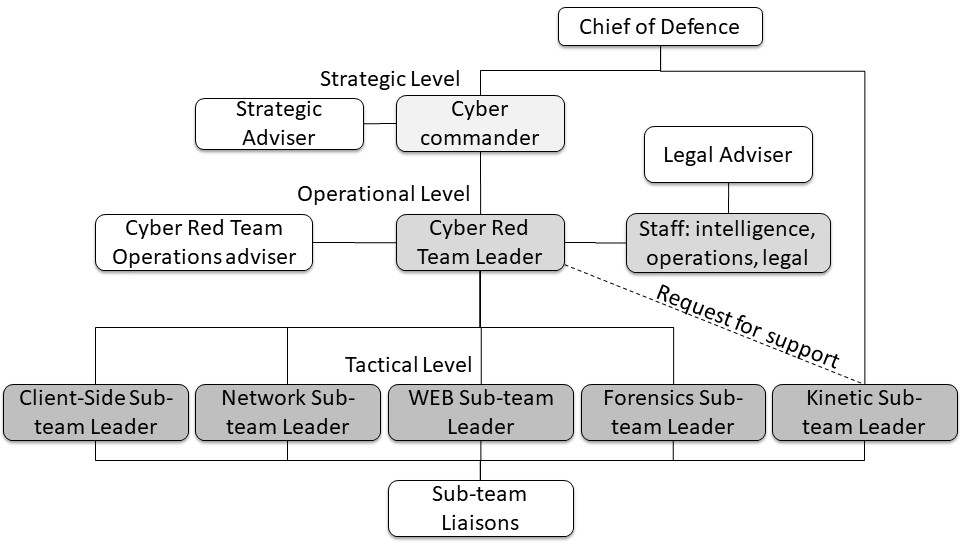
\includegraphics[width=1.0\textwidth]{./img/rt-org.jpg}
    \caption{``Crossed Swords 2019'' cyber red team chain-of-command}
    \label{fig:rtorg}
\end{figure}

These teams are subdivided into sub-teams according to the specialization and operational management level:
\begin{enumerate}
    \item \textbf{Red Team}: being the largest team of around fifty experts consists of exercise training audience. The chain-of-command and various sub-teams are the following:
    \begin{enumerate}
        \item \textit{Cyber commander.} The top-level officer in charge of commanding the cyber operation at a political level. This position is offered to the commanders of the NATO member nation cyber commands. Cyber commander, as part of the training audience, manages and coordinates the cyber operation to reach the set mission goals and coordinates the high-level activities, based on the desired effects, of the sub-teams. Even if the role of the exercise cyber commander might be underestimated it serves as a learning opportunity to the commander on how such cyber-kinetic team would be managed, how to coordinate the activities whilst maintaining the situational awareness. Additionally, this serves an experience for the technical cyber-kinetic team members to always have a clear understanding of the higher commander intentions, provide the situational reports in an understandable manner, and suggest course-of-action options for the mission objective accomplishment;
        \item \textit{Strategic adviser.} Is a member of the exercise development and management team (WT) with the role to provide the advice to the cyber commander, and, if needed, give minor hints to keep the red team activities on the course of designed scenario, as much as it is possible. This option allows exercise developers to explore the nuances and alternative paths for the developed scenario, allowing deviations as long as the end result objectives are met;
        \item {Red team leader group.} This small group of experts, operating at a strategic level and under direct command of the cyber commander, are responsible for fulfilling assigned operational effects by working with the sub-team leaders and ensuring that objectives, force protection, and intelligence activities are correctly executed and reached. This group consists of three experts: the overall red team leader, \gls{opsec} officer, and an intelligence officer;
        \item \textit{Sub-team leaders.} The main red team consists of five expert-focused sub-teams, at a tactical level, which are represented by their leaders. The purpose of every sub-team, consisting of up to ten experts, is to deliver the intended effects at their responsibility area by performing covert infrastructure maintenance, asset protection, stealthy attacks, infiltration of adversary's information systems, precision take-downs, information extraction and gathering, adversary assessment, and cyber-kinetic engagements. Over the exercise iterations it has been identified, that the most applicable size, ensuring its management and providing required capability, of the sub-team is from six to ten experts.
        The role and purpose of every sub-team is as follows:
        \begin{enumerate}
            \item \textit{Client-side attack sub-team.} This team focuses on executing attacks targeted at exploiting end-user (i.e., human vulnerabilities) to get the initial foothold, such as, creating a \textit{spear-phishing} campaign, setting up \textit{watering-hole} or \textit{drive-by} attacks. Once initial breach has succeeded this team performs privilege escalation by exploiting the vulnerabilities on the target client operating system (e.g., MS Windows, GNU/Linux), perform MS Windows domain take-over, conduct lateral movement, control critical processes, such as, unmanned aerial or ground vehicle management graphical user interface, and ensure persistence in the target computer network;
            \item \textit{Network attack and exploit development sub-team.} The goal for this team is to target exposed computer network services, gain control over them by abusing the misconfiguration, poor implementation, abuse, or developing and exploiting software vulnerabilities. Additionally, this team is conducting IP network (IPv4 and IPv6) and service mapping, and executing attacks against specialized systems, such as, tactical radio networks, mobile operator base stations, and \gls{ics} elements;
            \item \textit{Web-application attack sub-team.} For this team all web-based systems and technologies, such as, web-applications, services, and back-end relational databases, are the target. This team extracts valuable information from the web-applications, such as, user credentials, e-mails, or application source code, as well as breaches the security of an exposed web-application to gain access to the internal network services, and establish persistence;
            \item \textit{Digital battle-field forensics sub-team.} The main effort of this team is to perform data carving and artefact extraction from various sources, such as, hardware devices (e.g., smart phones, portable computers and other electronics), computer memory or hard disk images, by applying digital forensics techniques. This team uniquely serves as the bridge between the cyber and kinetic operational components as it is tasked to perform analysis of forensic evidence extracted either by the cyber sub-teams or brought in from the field by the kinetic team. The goal of the forensic team is to extract valuable evidence or information, such as, intelligence information, sensitive documents, malware command and control server addresses, passwords, or enemy communication channel encryption keys; and
            \item \textit{Kinetic forces sub-team.} This team formed from trained military and law-enforcement experts performing various kinetic operations, such as, forced entry, covert access, hardware extraction, target capture or take-down, intelligence collection, surveillance, or kinetic activities on enemy territory. The interaction between the red team provides the one of the key aspects for cyber-kinetic game-play and operation execution. This team is managed and trained by industry experts (e.g., HTCI -- High-Tech Crime Institute) and \gls{sof} instructors. The created scenario is designed to have the interdependencies within the red team and anticipates the cyber-kinetic cooperation. For example, the cyber red team might identify a lead, by collecting and assessing the digital evidence, to a crucial asset, such as, air-gapped server containing adversary communication encryption keys, which is not directly reachable by cyber means and requests the kinetic force engagement for planning and executing the operation to acquire it. In this example, the kinetic force is trained to identify needed hardware, learn its extraction techniques, and preserve digital evidence. Also the kinetic force team might depend on cyber team's support, for example, when executing a forced entry into adversary's data centre protected by a blast-door this can be either can be achieved either by kinetic attack (e.g., use of explosives or physical force) or by cyber means (e.g., targeting the ICS/SCADA system controlling the doors or cutting the power to trigger fail-safe procedures). In this example, depending on the entry method, the kinetic force team might have less or more time to perform the intended activities.
        \end{enumerate}
        \item \textit{Sub-team liaisons.} For every mentioned sub-team there is an attached WT liaison responsible for observing and, if required, providing minor hints to the sub-team leader to ensure that the team is not wasting too much time on some targets, such as, cyber decoys and honeypots, and does not deviate from the intended scenario too much; and
        \item \textit{legal advisers.} With advisers embedded to assist every level -- political, strategic, and tactical. The role of these experts is to provide their assessment of the activities form the international and domestic law perspectives. They are not allowed to break the game by denying certain actions, but more giving an insight to the participants on legal implications and consequences of their activities. These experts are heavily used by the training audience to verify and confirm the legality of their planned actions and choose the one compliant or with least consequences. This gives not only the experience and comprehension of ramifications for various taken activities to the technical members of the red team, but also the training experience to the legal advisers as they have to tackle the questions and situation which they might not encounter on day-to-day basis.
    \end{enumerate}
    \item \textit{Blue Team.} Is a small team of up to four experts experienced in conducting cyber red team activities. This team is under direct control and supervision by the white team and is used to manage the cyber red team's progression within the adversary's computer networks. The main tasks for this team are user and adversary simulation. As a user simulation role-player, they are directly engaged in client-side conducted activities, such as, examining and deciding to open received malicious attachments, visiting the web links, or browsing the in-game web services. With this role their task is to observe, assess and deny or permit the cyber red team's initial foothold, based on the quality and delivery method sophistication level. As an adversary simulation team, their task is to detect the cyber red team's presence, related \gls{ioc}, assess the scale, sophistication and red team objectives, and, if permitted, compromise the red team operational infrastructure in a counter-red team operation. By adjusting the level of the resistance of the adversary's information system the cyber red team will have to take this into account when executing their attacks, maintaining \gls{opsec}, and protecting their assets;
    \item \textit{White Team.} Is a small group of experts, typically no more than two, responsible for controlling and steering the exercise according to the developed scenario. As mentioned before, deviations from scenario are accepted and some-times encouraged, as long as, the overall focus is not lost, and mission objectives can be reached. It has to be noted, that the exercise does not have the ultimate goal of succeeding in accomplishing the intended scenario and fulfilling entirely the laid mission goals by any means necessary. Depending on the activities pursued by the red team, their course-of-action and time limitations, the mission might be a failure, as it can happen in real life. Within the past iterations of the exercise the red team only once successfully accomplished all of the laid mission objectives, and in other cases completing them partially.
    \item \textit{Yellow Team.} This team, composed of experts, focuses various areas of threat and anomaly detection, such as, monitoring, big data analytics, intrusion detection, and situational awareness. The tasks and produced results of this team are described in more detail in chapter \ref{sec:feedback}. The most crucial task for this team is to provide the near-real time situational awareness picture to the red team, which represents how the red team operation looks, the detected tools, made mistakes, and identified \gls{tttp}. This fed-back allows the cyber red team to immediately spot the made mistakes and adjust their operations and tool usage to avoid the detection, therefore not only increasing the level of stealth, but also having a better understanding on the used tools and performed actions; and
    \item \textit{Green Team.} Is responsible for tasks, such as, maintaining the cyber range platform, supporting the game network technical requirements, developing the game network hosts and targets, and integrating new technologies either virtual or physical. The game network and introduced technologies are explained in more depth in chapter \ref{sec:scenario}.
\end{enumerate}

The described full-spectrum cyber operation execution, tasking, and command structure represents the technical and human environment with its various interdependencies and nuances, where the current work from the listed publications has been implemented and assessed. This includes:
\begin{enumerate}
    \item Red team -- uses the proposed \gls{tttp}, if they are applicable for a particular objective or to deliver the desired effect. Gaining initial access by developing a custom exploit or fuzzing a proprietary network protocol (\ref{pub:secondPub}) has been successfully executed by the cyber red team against the developed in-game target systems, such as, finding a vulnerable command in a designed network service, allowing stack-based memory buffer overflow exploitation and target system take-over. Established initial foothold on a dual-stack host allows the \gls{cnc} channel establishment back to the red team's operational infrastructure attacking hosts, for specific tasks, such as, covert information exfiltration or individual high-value target system control the custom covert channels have been successfully established (\ref{pub:firstPub}). In addition to these tools, the red team extensively uses also third-party collaboration and post exploitation frameworks (e.g., Cobalt-Strike, Empire, Pupy), which rely on traditional protocols used for \gls{cnc} communications, such as, HTTP, DNS, and SMB. However, when compared to the proposed \textit{nc64} capabilities, these typical channels are relatively easily detected by the yellow team, and the red team has to make sure, that they are properly configured and adjusted to minimize their detection. For such channels, for example, the compliance with expected protocol payloads have to be ensured not to be easily distinguished from the overall traffic, the beaconing (i.e., call-back) timing and randomization has to be considered to avoid behaviour pattern-based matching and used \gls{cnc} protocols have to make sense for the target hosts. The \gls{ics} oriented zero-day development (\ref{pub:thirdPub}) has been implemented in the game environment, and the red team is faced with identifying weaknesses and exploiting them. All of the described attack vectors in that publication have been successfully also transferred into the exercise and cyber red team has developed the exploits under supervision of an instructor. Due to exercise time restrictions, the instructor gives some leading hints in form of a question allowing the training audience to understand and successfully accomplish the goal within a reasonable time frame. For example, the PROFINET IO attack has been used to control the adversary's data centre bunker doors, and IEC-104 and Martem RTU attacks -- to disable the enemy's military base power supply;
    \item Adversary simulation team (BT) -- it is not mandatory for this team to use any of the proposed cyber-red team oriented \gls{tttp}, as for the adversary simulation team it is not the main purpose of remaining undetected. In some cases, the techniques and tools as described in \ref{pub:secondPub} have been used against the cyber red team's operational infrastructure, but in most cases the red team \gls{opsec} failures are used against themselves, such as, unchanged default passwords on the attacking machines, not removed metadata in the delivered infected documents, or leaving unattended back-doors;
    \item Legal advisers -- according to the scenario, as introduced in the following chapter \ref{sec:scenario}, the artificial conflict tackles both international and domestic law. In cases, when international law applies, the work in \ref{pub:eighthPub} is used to consult the situation and assess its legal implications;
    \item Yellow team -- to provide the near real-time feedback and situational awareness picture, as described in detail in chapter \ref{sec:feedback}, the solutions for Syslog data aggregation, parsing and correlation (\ref{pub:fourthPub}, \ref{pub:fifthPub}) are used alongside with the other technologies allowing threat detection and visualization. The cyber red team has to be trained to identify the cyber deceptions and honey-pots (\ref{pub:sixthPub}), therefore a set of various honey-pots (e.g., low- and high-interaction, and adaptive) and decoys with planted \textit{breadcrumbs} are placed within the adversary's computer networks. This serves not only as a method to represent the situational awareness to the red team but attempts to teach the experts that not all systems have to be targeted and how to identify the decoys. The \textit{Frankenstack} framework (\ref{pub:seventhPub}), consisting of multiple interconnected tools and solutions, is the core solution developed by the yellow team to provide near real-time situational awareness to the cyber red team; and
    \item Green Team -- to make the exercise challenging, technically interesting and represent real-life systems as much as possible, the research results (\ref{pub:thirdPub}) are adapted and re-implemented from real cyber operations. The goal for such system integration is to give opportunity to the red team to practice attacks against real systems, which are not available to the participants on day-to-day basis. The introduced technical challenges are covered in more detail in the upcoming chapter \ref{sec:scenario}.
\end{enumerate}

\subsection{Technical Environment, Exercise scenario and Legal Considerations}
\label{sec:scenario}
\textbf{Technical environment and scenario.}
The ``Crossed Swords'' (XS) exercise game network is hosted on a cyber range running VMware ESXi hypervisor and it consists of around 200 virtual machines for in-game core networking, simulated Internet, cyber red team segment, and a set of target networks. Not all intended technical game-play elements can be virtualized, therefore the game network is expanded by connecting physical hosts and systems through the cyber range infrastructure. Before creating the overarching geo-political scenario, the technical scenario is established based on the core development team ideas and intended technical game-play intentions.
Due to XS being relatively small, with respect to the game-network scale and training audience size, experimentation and introduction of new, recently prototyped, and orthodox technologies can be afforded making the technical game-play more attractive and as close to the real-life as possible. The network also uses the traditional \gls{it} systems to provide the networking and common workstation operating systems, such as, MS Windows and GNU/Linux, to provide replicate the structure of a regular office and business networks.
The following list briefly summarizes some of the technologies introduced in the XS game series, to highlight the technical level:
\begin{enumerate}
    \item Bunker door -- a system, running a set of interconnected Siemens developed S7-1200 \gls{plc} based PROFINET IO-devices, is controlling the bunker door. The cyber red team has to analyse and reverse-engineer the PROFINET IO RT protocol to inject remotely the commands to open or close the bunker door;
    \item Alarm system -- a bunker door is protected by the Paradox supplied alarm system and, before the door can be opened, the alarm system has to be targeted remotely by analysing the used bus-protocol, and capturing and decoding the PIN code;
    \item CCTV IP camera -- attack implies the cyber red team finding and exploiting the flaws in the actual IP-based surveillance camera web interface to gain full control remotely;
    \item Distributed power-grid -- a system based on IEC-61850 and IEC-60870-5-104 industrial Ethernet protocol series and a Martem produced \gls{rtu} is used to manage and supervise the distributed power-grid. The red team has to reverse-engineer the IEC-104 protocol and perform remote command injection to control the power supply either by turning it off or on;
    \item Anonymization network -- red team has to infiltrate the real \textit{i2p} anonymization network to intercept and modify the \gls{cnc} communication channel running over that network;
    \item Unmanned aerial vehicle (UAV) -- adversary's Threod manufactured UAVs, flying over or approaching the protected territory, have to targeted to gain control over the provided video stream, taking over the steering, or destroying the UAVs;
    \item Unmanned ground vehicle (UGV) -- Milrem developed UGVs serve as an adversary-controlled tank force and the cyber red team is tasked to take full control over them by targeting either the used network protocols or the controlling workstation;
    \item Maritime navigation -- a vessel's steering and tracking system based on the OTH-GOLD (Over-The-Horizon GOLD) and AIS (Automatic Identification System) maritime protocols is targeted by the red team to gain control over the ship and inject naval tracks to confuse the situational awareness;
    \item Radio communication network -- the network based on Harris constructed military-grade radio stations has to be infiltrated by the red team via extracting the encryption keys for the communications running over the radio carrier;
    \item Mobile network base stations -- the cyber red team has to infiltrate the LMT (Latvian Mobile Telephone) operator provided base stations connected to the actual mobile network, analyse and parse the intercepted communications to decode the adversary agent's message exchange (SMS) and pinpoint their physical location;
    \item Mobile 4G network -- red team is tasked to gain access to the Ericsson developed 4G mobile network equipment and execute further attacks against connected nodes;
    \item Railroad control station -- a system based on Siemens created S7-1200 \gls{plc}, running s7comm+ protocol, is used to control the in-game railroad network. The red team is tasked to gain control over the railroad control stations either to stop or derail the train; and
    \item Environment monitoring wireless sensors -- the red team has to control the Defendec provided Smartdec wireless sensors to track the physical location of an adversary troops.
\end{enumerate}

The various technical challenges implemented across nearly all of the game-net systems, are designed in a way, that no single sub-team of the red team can solve them on its own. To achieve this, cooperation, information exchange, objective tracking, and operation management is emphasized to provide the collaborative training experience and attempting to push the participants out of their comfort zones. The technical scenario, being time limited and fast-paced, cannot be fully solved, therefore the cyber red team has to consider ways and approaches on how to prioritize the technical objectives and manage the focus of force to accomplish the overall mission objectives within the exercise time.

The integration of real-life vulnerabilities and systems, such as, the ones as described in \ref{pub:thirdPub}, deliver the learning perspective to the exercise participants. Examining, developing exploits, and attacking the systems which are widely used for automation and industrial process control are challenging and allow the training audience to comprehend the actual state of security for such industrial components. Furthermore, some participants might have such systems in their organizations, but are not allowed to executed attacks or tests due to them being in a production state.
Cyber red team members, with some guidance by the instructors, follow the full weakness identification, vulnerability determination, and exploit development life-cycle as described in the chapter \ref{sec:impact}. Such approach has allowed the participants to successfully exploit the industrial control protocols and devices (\ref{pub:thirdPub}).

\textbf{Exercise scenario.}
The technical scenario, describing the interdependencies, attack vectors, and alternative paths, only covers the part for the actual work to be conducted by the exercise participants. To deliver the context, reasoning, and clear objectives, the overarching scenario is required. This scenario provides the elements, such as, the state-of-the-world background, geo-political situation, intelligence information on what has happened, what is the impact suffered, why the response is being triggered, what are the objectives and rules of engagement.
The main geo-political story revolves around a fictitious group of Cyberbian islands, where every island is a country with its technological advancements, political stance, alliances, and intentions. The three island-countries are Berylia, Crimsonia, and Revalia. Berylia being the smallest with a modest military force, part of NATO alliance, and its main economic income originating from the electronics manufacturing. Crimsonia is the largest island with a strong military, rich in natural resources, not part of any alliance, and is expressing some signs of aggression against its neighbouring island-countries. Revalia is a small, self-sustained, and politically neutral country. Within the scenario, the exercise participants assume the role of Berylian rapid response team, which is assembled to address the looming crisis, maintain the resiliency of the national critical information infrastructure, and accomplish the mission goals.
Every year, with a new exercise edition, the scenario evolves and the tensions between Berylia and Crimsonia have been escalating, ranging from Crimsonia conducting a series of debilitating cyber attacks against Berylian \gls{cii}, abuse of a neutral nation infrastructure for operation conduct, placing insiders and double-agents, forming military blockades, up to launching a military invasion of Berylia. The various levels of conflict are designed to explore the technical, cyber-kinetic, and legal game-plays as every particular state opens new opportunities and provides flexibility in conducting the responsive computer network operations. The operational environment for the kinetic force's unit is extremely important, as this restricts, or enables, some types of activities to be exercised.

\textbf{Legal considerations.}
A part of the exercise scenario consists of legal game-play. Despite the exercise not having legal aspects as the primary objectives, the legal guidance and considerations are incorporated in the form of legal scenario injects aimed to trigger the discussion and legal implication consideration during the situational report meetings. Legal advisers are assigned to every level of the chain-of-command to assess and consult the exercise participants. 
The legal aspects of the conducted cyber-kinetic operations and applied \gls{tttp}, within the context of the scenario, tackle at least the following legal considerations as covered in \ref{pub:eighthPub}:
\begin{enumerate}
    \item \textit{Applicable law (Part II)}.
    Depending on the circumstances ruling at the time, the lawyers are tasked to ascertain which regimes of public international law apply to the cyber operations occurring during the exercise. The cyber attack campaigns of the exercise range from those occurring in peacetime to those endangering national and international security. The storyline generally avoids situations of armed conflict. The exercise scenario attempts to bring all of the five operational domains (i.e., land, sea, air, space, and cyber) into the game-play, extended by espionage, and cyber-kinetic operations. Such activities may be addressed by the international human rights law, diplomatic and consular law, law of the sea, air law, space law, and international telecommunications law;
    \item \textit{States entitled to take countermeasures (Rule 24)}. Only state affiliated institutions and organizations, such as, military or intelligence, can conduct responsive activities on the state's behalf as long as the activities they engage in do not constitute an internationally wrongful act. The cyber operations by private entities, such as, business companies or non-governmental organizations (NGO), can never constitute countermeasures in the legal sense. Therefore, the players assume the role of a rapid response team, assembled  on the order of Berylian government, which is placed under the supervision of the military command;
    \item \textit{Effect of \gls{rcd} on third parties (Rule 25)}. Due to the fact that \gls{rcd} has extraterritorial nature and implicates pursuing the adversary, as well as, performing malicious service take-down within the cyberspace, the legal advisers are required to assess the legality of the \gls{rcd} effects on the third parties. These activities may include operations, such as, third-party \gls{vps} take-over, hacking adversary controlled \gls{cnc} servers on the Internet, back-dooring or re-weaponizing the malicious code used by the adversary and compromising public web services to plant the targeted exploit-kits. Since such operations are intentional, both from the adversary and defender side, they have an effect on third-party owned systems or against ones residing in a neutral state (i.e., Revalia). For the red team to complete their mission objectives, the \gls{rcd} activities have to be deemed lawful, the various possible paths have to be explored, their effects evaluated, and necessary precautions taken, if such are reasonably possible;
    \item \textit{Limitations on \gls{rcd} (Rules 23, 26, 72, 73, 113)}. Depending on the legal qualification of the \gls{rcd} operations, various limitations, such as, concerning necessity, proportionality, imminence and immediacy, are attached to this operation. The legal advisers are tasked to identify any applicable limitations, such as, requirements for the \gls{rcd} to be necessary and proportionate, and provide these legal implications to the commander or sub-team leaders. The scenario addresses both the cyber and kinetic attacks and activities performed by the adversary against the defended state and its \gls{cii}. Those include malicious operations, such as, serious cyber attacks, espionage, sabotage, and deployment of malware (e.g., condition-activated logic-bombs) with the goal to debilitate the state's critical services and capabilities. Adversary's kinetic activities include operations, such as, armed drone attacks, navy blockades, placement of a large amount of troops on the borders, and expeditionary force deployment. The game-play is initiated by the series of escalating events leading to ongoing or imminent threat, which may serve to prove the necessity of the taken responsive operations, which are evaluated by their proportionality and delivered effect.
    As derived from the scenario, the defending state has to immediately respond to an ongoing or imminent threat to ensure the resiliency and protection of critical assets relevant to the security, functionality and well-being of the state;
    \item \textit{Self-defence against an armed attack (Rule 71)}. The scenario is designed in such a manner that the severity offensive action against the victim state amounts to to an armed attack, thus permitting to respond in self-defence with an immediate asymmetric responsive cyber operations against a stronger and advanced adversary. The scenario can be designed more subtle and with less tensions, however, in such case the training audience would struggle proving the necessity to pursue the adversary and infiltrate their network, which would have an impact on the overall game-play and achieving the currently set mission and training objectives;
    \item \textit{Geographical limitations of cyber operations (Rule 81)}. The effects of a cyber operations have to be limited to the intended target information systems and geographical locations. This, although not always being possible to limit geographically, is taken into consideration by the red team when executing the cyber operation which may include the activities, such as, placement of drive-by exploit-kits on third-party services. The red team might not be aware of geographical location of a targeted asset in cyberspace, however, when such attack campaign is executed, measures are taken to restrict its spread within the intended target's network address ranges if it is possible;
    \item \textit{Means and methods of cyber warfare (Part IV, Chapter 17, Section 5)}. The exercise scenario plays on the various levels of aggression and conflicts without entering the state of war. Despite cyber warfare not being applicable directly it is still to be considered and applicable methods have to be evaluated accordingly, since, within the played-out high-tension scenario, it could unexpectedly escalate to an armed conflict and the state of war;
    \item \textit{Precautions (Part IV, Chapter 17, Section 7)}. For the executed cyber operations, the red team is asked to exercise constant care, perform verification of targets, choice of means or methods, choice of targets, evaluate proportionality, and estimate the effects of cyber attack whenever it is reasonably possible and applicable;
    \item \textit{Cyber operations in neutral territory (Rule 151)}. The adversary may proxy their cyber attacks or route the kinetic attack, such as, drone flying through neutral state's air space before heading to the intended target. In such cases, the red team's response might have uncertainty and limitations on taken actions in the neutral state's cyberspace. The red team might be tasked with pursuing alternative paths or collecting more attribution evidence, before executing cyber operations within the targets in neutral state's cyberspace; and
    \item \textit{False-flag and no-flag operations.} For the red team to protect their identity, assets and intended objectives, a false-flag or no-flag operation would be considered to be executed to imply uncertainty and make attribution harder. From the technical perspective, the cyber red team might adapt the known \gls{tttp} of a chosen threat actor to deceive the adversary. From the legal point of view, it is not clear if such operations are permitted when, for example, impersonating and adversarial profile of a threat actor with high certainty attributable to a third state.
\end{enumerate}


\subsection{Training Assessment and Real-time Feedback}
\label{sec:feedback}
One of the key aspects of the ``Crossed Swords'' exercise is to provide the environment, where the cyber red team can experiment, practice applicable \gls{tttp} and observe their effects in near real-time. Such opportunity provides the necessary feedback to the exercise participants for their tool and procedure stealthiness and efficiency, as well as, to the exercise management to evaluate the progress of the red team and the fulfilment of training objectives.
To accomplish this, a dedicated framework, called the \textit{Frankenstack} and described in \ref{pub:seventhPub}, is developed to deliver the required visibility through meaningful visual means and notifications.

The \textit{Frankenstack} development is facilitated and coordinated by NATO CCD CoE since 2016, with a group of an international team of experts. The development team is assembled from technical experts in the field of monitoring, data visualization, threat detection and assessment, and big data analytics. The contributions include NATO CCD CoE partners, such as, Arc4dia, Stamus Networks (Suricata IDS), Greycortex, Cymmetria, Tallinn University of Technology, CERT.LV, and CERT-EE.
The \textit{Frankencoding} events\footnote{Frankencoding. \url{https://github.com/ccdcoe/Frankencoding}. Accessed: 23/11/2018} have resulted in an ongoing \textit{Frankenstack} development with its source code released publicly\footnote{Frankenstack. \url{https://github.com/ccdcoe/frankenstack}. Accessed: 23/11/2018} on GitHub under the MIT license.

\textbf{Goals and design principles.}
The operational principles of the developed framework are defined as follows:
\begin{enumerate}
    \item \textit{increase stealthiness} of the red team executed operation, by providing comprehensive and real-time situational picture;
    \item \textit{improve \gls{rt} coordination} through granular multi-layered view of the detected attacks;
    \item \textit{analyse \gls{tttp}} and allow the red team to identify the weaknesses and improve the operational performance;
    \item \textit{open-source} tool usage as the building blocks for the \textit{Frankenstack} to lower the needed costs and increase the framework maintainability;
    \item \textit{customizable} and interchangeable open-source modules to be replaced for more efficient operations or introduced to expand the existing functionality;
    \item \textit{high automation} demands to minimize the latency introduced by human-in-the-loop, by applying solutions, such as, data clustering and pattern mining algorithms;
    \item \textit{real-time} provision of the identified threats to allow the adjustment of the red team campaign in a timely manner;
    \item \textit{transparency and visibility of actions} delivering the processed information for further analysis at different levels, such as, host-based, or network-based, to the red team members;
    \item \textit{adequately detailed} information to be provided to the red team not experienced in system monitoring or data analysis, while still providing enough detail in line with the current game-play progress of the red team; and
    \item \textit{correlated attack visualisation} to make the detected attacks and threats easily understandable to the exercise participants, exercise control, and observers. This has been implemented by a novel web-based Event Visualization Environment (EVE) and displaying the detected attacks on an interactive network map.
\end{enumerate}

\textbf{Integration in the game network.}
The solution is easily deployable in the game network and can accept any possible sources of information to be further processed, which can be from at least the following origins:
\begin{enumerate}
    \item \textit{ERSPAN (Encapsulated Remote Switched Port ANalyser)} traffic mirror collecting all the network data recording, parsing, and deep packet inspection;
    \item \textit{NetFlow} from game network routers for traffic statistical analysis and evaluation;
    \item \textit{data from the systems}, such as, system performance metrics (e.g., CPU load, HDD utilization, network interface card statistics), and logs (e.g., Syslog, and application textual log-files);
    \item \textit{honeypots and cyber decoys} placed in the network to attract and deceive the cyber red team into revealing its \gls{tttp}; and
    \item \textit{aggregates the information from all sources} in textual format allowing this to be reduced to a log correlation and analysis problem.
\end{enumerate}

\textbf{Assessment.}
During the ``Crossed Swords 2017'' execution the members of the white team performed the assessment of the deployed \textit{Frankenstack} solution for its usefulness and training benefits. The identified findings were addressed and incorporated into the following exercise editions. The conducted expert qualitative interviews and online survey results reflected the following:
\begin{enumerate}
    \item the deployed tools themselves do not increase the learning perspective, but is up to how red team members perceive and use the tools;
    \item the addition of situational awareness solutions to the exercise is welcome and seen as a necessary component;
    \item the four large screens in the execution room, showing the yellow team provided information, was preferred and checked approximately every 45 minutes by the majority of the training audience;
    \item exercise participants also used the opportunity to access the \textit{Frankenstack} dashboards locally on their computers and dig deeper when attempting new attack vectors;
    \item \textit{Alerta} tool, showing the identified attacks as priority categorized alerts, was found most useful by the majority of the trainees;
    \item it was acknowledged, that ease of use should be further improved especially when considering the merger of high intensity technical exercise with monitoring tools not known to all participants;
    \item majority of the training audience strongly agreed that the provided situational awareness was beneficial to the learning process, was accurate and delivered in acceptable speed;
    \item the larger part of the training audience agreed that they learned more regarding how their actions can be detected and tried to be stealthier; and
    \item integration of various tools into the \textit{Frankenstack} has to be evaluated carefully to avoid visual distractions and making the output more self-explanatory.
\end{enumerate}

\subsection{Chapter Conclusions}
The technical exercise ``Crossed Swords'', created and led by the author, integrates all of the research from the listed publications to deliver the innovative and novel training environment for the cyber red team. The flexibility and agility of the exercise permits it to be used as a platform for experimentation, research, and verification of new ideas and concepts. By exploring yet not fully understood concepts of cyber red team assembly and structure, cyber operation management and execution, \gls{tttp} applicability and stealth, near real-time feedback, and intense game-play scenario, permits to identify and verify the functional aspects of cyber operation nuances, which can be integrated into actual cyber operation execution.
The exercise strives to provide to the training audience the increased and recognized training experience and benefits by combining the technical, operation management, and legal aspects. The conducted survey (see appendix on page \ref{app:survey}), with an intention to gather overall feedback and impressions from the exercise participants since year 2014, identifies the learning benefits acknowledged by the training audience.
The unique near real-time feedback, delivered to the cyber red team via the \textit{Frankenstack}, permits the team members to assess and increase their skills, employed techniques and tools, adapted tactics and procedures, and promotes deeper understanding of the situational awareness and cyber red team executed responsive computer network operation.



\section{CONCLUSIONS AND FUTURE WORK}
\label{sec:end}
\glsresetall
\subsection{Summary and conclusions}
This thesis addresses the lack of public information, understanding, and knowledge on the responsive computer network operation execution within the recently recognized domain of cyber operations. As well as, explores the cyber red teaming applicability to such operation execution, operational asset protection, and required training for the cyber red team. Thesis examines three main closely tied concepts: (1) cyber red team capabilities, novel \gls{tttp}, and engagements in responsive computer network operations; (2) utilization of anomaly detection and cyber deception novel methods for adversary tracking, situational awareness, technical attribution, and red team asset protection; and (3) cyber red team oriented technical exercise design, structure, execution, legal implications, and novel near real-time feedback provision to the training audience.

Chapters \ref{sec:crtopreq} and \ref{sec:crtops} identify and define the building blocks to determine the definition for specialized cyber red team computer network operations. The author addresses the inconsistency and variety of definitions for the concepts of \gls{rcd}, \gls{cno}, and \gls{crt}, and defines a new concept of specialized \gls{crt} responsive \gls{cno} applicable throughout the thesis. As well as, the main characteristics of such operations are estimated. The work in related publications (\ref{pub:firstPub}, \ref{pub:secondPub}, \ref{pub:thirdPub}) is assessed from the perspective of novel \gls{tttp} development applicable to the responsive computer network operation execution by the cyber red team. These techniques and tools are compared and evaluated alongside with other popular and commonly used solutions to elaborate the advantages of the proposed ones. The novel \gls{tttp} are mapped against the identified characteristics of specialized \gls{crt} responsive \gls{cno}, to present their suitability for such operation execution and designated effect delivery.

When considering the specialized cyber red team responsive computer network operations, their extraterritorial nature and offensive capacity has to be acknowledged. For the \gls{crt} to identify, track, and pursue the adversary within the cyberspace, the red team would, to a certain extent, follow the cyber attack execution phases (e.g., reconnaissance, initial foothold, command and control). Such phases, from the defender's perspective, are mapped to a cyber kill-chain, allowing to identify and possibly stopping the incoming attack at every stage of the kill-chain. When assessing the popular and accepted cyber kill-chain methods (e.g., Lockheed Martin, Microsoft, Mandiant/FireEye), it can be seen, that there are areas, where a particular method is stronger or weaker. To address these gaps and emphasize the strengths, a new unified model of ``cyber attack kill-chain'' is proposed by the author. For the \gls{crt} to increase the chances of success, the proper techniques for countering the detection at every phase of the cyber attack kill-chain need to be identified. The proposed cyber red team novel \gls{tttp} are mapped against the cyber attack kill-chain to identify their applicability on countering or supporting it at most of its stages.

Chapter \ref{sec:protection} explores the effects granted by the novel anomaly detection and current cyber deception solutions and approaches. These methods are explored from the perspective on how they can benefit the cyber red team conducted operations. The novel system log file based anomaly detection and cyber deception techniques are evaluated to grant the \gls{crt} the needed scalability, efficiency, ease of automation and management. These approaches fit into the \gls{crt} life-cycle and provide the solutions required for passive defence, syslog analysis, attack surface spoofing, honeypots, cyber decoys, and tarpits. From the delivered effect point of view, the proposed techniques help to detect, deceive, disrupt, degrade, deny, and defend against the adversarial activities.
The responsive \gls{cno} executed by the \gls{crt} would require some form of infrastructure to operate from. This operational infrastructure, depending on the tasks and set objectives, can be used to conduct at least the minimum set of the response related activities, such as, target reconnaissance and vulnerability assessment. The proposed conceptual model for the \gls{crt} operational infrastructure includes the following logical network zones -- cyber operation execution area (location and initial origin of the cyber red team), support area (location, where attacking hosts are deployed with the attack execution supporting resources), staging area (network hosts used to directly interact with the target information system), command and control area (where the \gls{cnc} servers are deployed), and the decoy area (hosting the decoys to where suspicious activity is redirected for further examination). Every particular area has the applicable detection and cyber deception solutions deployed to allow the \gls{crt} maintain the visibility over the deployed technical assets, provide means for adversary tracking in case of a possible counter operation, and contribute to increasing the operational security.

Chapter \ref{sec:exercises} examines the use case of the created and developed technical exercise ``Crossed Swords'' aimed at training the cyber red team in a close to real-life conditions. This exercise integrates all of the listed research work and publications by the author and indirectly serves as the test-bed for novel research conduct and result verification. Besides primarily being a technical exercise, also cyber red team management, leadership, information exchange, and legal issues are tackled, to provide the training experience as close to the real cyber operation execution as possible. One of the corner-stones for the exercise is to explore the cyber kinetic interactions by integrating military units (e.g., special operation forces, military police, and army) into the operational game-play. Such kinetic force game-play is intertwined with the cyber operation to find the synergies, where mutual benefits and cooperation can be identified, emphasized and exercised.
The training audience, assembled into the \gls{crt} and pursuing the assigned mission objectives, practices the existing and novel \gls{tttp} for situational awareness, attribution evidence gathering, target identification, target information system covert infiltration, stealthy activities, and mission objective completion. For this to be successful, a near real-time situational awareness is provided to the participants by the means of novel collection of monitoring, threat detection, and visualization solutions, called the \textit{Frankenstack}. This information gives a timely feedback to the participants to observe the reasons behind the detection of the conducted attacks and allows to identify the needed improvements to increase the level of stealth.

% Research questions and answers to them
\subsection{Answering the research questions}
Each of the research questions is answered by providing the answers to the respective sub-questions.

\textit{[Q1.] What are the specialized cyber red team technical capabilities for responsive computer network operations?}

\textit{[Q1.1.] Which features the techniques, tools, tactics and procedures have to possess to be applicable to the specialized cyber red team responsive computer network operation requirements?}
The identified characteristics of the specialized cyber red team computer network operations include at least the following ones: stealthy and innovative, agile and available, targeted and pervasive, rapid and timely, integrated and coordinated, hybrid and effective, and asymmetric.
The applicable techniques, tools, tactics and procedures have to support these operational characteristics as much as it is possible.
The innovative tools developed based on the suitable techniques have to be at least available on demand, customizable, increase stealth, support asymmetric response, and allow targeted focus of force. This thesis introduces multiple techniques for initial target network access, command and control channel establishment, and impact delivery, which have resulted in the prototyped tools (\textit{tun64}, \textit{nc64}, \textit{Bbuzz}, \textit{iec104inj}, and other proof-of-concept scripts). The suitability of these tools is assessed by comparing them to other relevant and common tools and solutions, and through conducting practical experiments. The results presented in the listed publications (\ref{pub:firstPub}, \ref{pub:secondPub}, \ref{pub:thirdPub}) and summarized in thesis chapter \ref{sec:scrtop} on page \pageref{sec:scrtop}, confirm, that the proposed techniques possess the required features and are applicable to develop suitable tools for specialized cyber red team responsive computer network operation execution, with appropriate tactics and procedures being applied. Furthermore, the proposed techniques and prototyped tools can be also applicable to a wider range of engagements, such as, penetration testing, cyber exercise development and execution, and related cyber operations.

\textit{[Q1.2.] How these proposed techniques, tools, tactics and procedures are suitable to counter the cyber attack kill-chain?}
To provide a more comprehensive cyber attack kill-chain, the existing recognized kill-chains are analysed and consolidated to introduce a new unified model attempting to cover all attack stages as thoroughly as possible. The proposed cyber attack kill-chain, introduced and described in chapter \ref{sec:killchain} on page \pageref{sec:killchain}, presents the following phases: reconnaissance, initial compromise and foothold, command and control, internal reconnaissance, lateral movement, privilege escalation, persistence, asset reconnaissance, and objective completion. For the cyber red team to increase the success of targeting and infiltrating the identified adversarial information systems, suitable \gls{tttp} have to be used to counter possible detection and operation disruption methods at every kill-chain stage. These techniques can be used to support countering all of the cyber attack kill-chain stages either by being directly applied or indirectly supporting other possible methods for countering that specific stage. This is accomplished through granting novel ways for initial compromise and foothold establishment, command and control channel creation, and targeting particular components of the information system. For example, methods for initial foothold can be applicable for gaining further access within lateral movement phase and attempting persistence. Also, established covert command and control channel supports all further activities performed within the target network starting from initial foothold up to objective accomplishment. As well as, targeted vulnerability identification techniques are applicable to support exploitation and privilege escalation attempts.

\textit{[Q2.] How to establish the situational awareness for the cyber red team?}

\textit{[Q2.1.] How system log file analysis and cyber deception approaches are relevant to cyber red team work-flow when executing responsive cyber operations?}
The novel system log file-based correlation and anomaly detection tools in combination with cyber deception solutions, as covered in chapter \ref{sec:protection} on page \pageref{sec:protection}, are applicable to specialized cyber red team responsive computer network operations. For such techniques to be relevant for the inclusion into cyber red team work-flow, they have to possess at least the following characteristics: readily-available and can be obtained by the red team on demand; easily deployable and manageable to lessen the administration overhead and conserve time; flexible and scalable, allowing to be adapted for operational requirements in various environments; highly automated to further reduce the system administration upkeep and human expert involvement; lightweight, permitting fast deployments and having low computing resource consumption requirements; and can be integrated with other technologies already present on the systems. The introduced novel log-based anomaly detection approaches and tested cyber deception solutions (\ref{pub:fourthPub}, \ref{pub:fifthPub}, and \ref{pub:sixthPub}) comply with the presented requirements and are applicable for introduction into cyber red team work-flow.

\textit{[Q2.2.] In what ways such solutions are applicable to situational awareness, red team operational infrastructure protection, and attack technical attribution?}
The chapter \ref{sec:opinfra} on page \pageref{sec:opinfra} introduces and explains the conceptual model for the cyber red team operational infrastructure, where the system log file-based anomaly detection and cyber deception solutions are deployed at various logical network segments. The placement of log analysis and deception tools within those network segments is clarified and their deployment reasoned. The primary goal of such techniques is to aid the cyber red team with providing at least the situational awareness, permit adversary tracking and threat assessment, conduct technical attribution, and protect the cyber red team assets. The proposed techniques and approaches confirm their applicability for cyber red team executed responsive computer network operations.

\textit{[Q3.] How to prepare and train the cyber red team for responsive computer network operation execution?}

\textit{[Q3.1.] What considerations are applicable for training cyber red team as close to the real-life conditions as possible in a technical cyber exercise?}
The chapter \ref{sec:exercises} on page \pageref{sec:exercises} explains and analyses the use case of the cyber red team oriented technical exercise ``Crossed Swords'' series (\ref{pub:tenthPub}).
The identified applicable considerations are at least the following: training environment providing freedom and flexibility to the exercise participants; cyber red team structure design according to the training objectives, mission goals, and cyber operation governance; clear chain-of-command establishment for progress tracking and effective cyber red team management and tasking; sophisticated technical challenges and game-network development, implementing real-life use cases and new technologies (\ref{pub:thirdPub}); appropriate over-arching scenario design to provide the reasoning for the responsive activity immediacy; appropriate technical solution and \gls{tttp} implementation (\ref{pub:firstPub}, \ref{pub:secondPub}, \ref{pub:thirdPub}) allowing to increase the level of stealth and execution speed; near real-time cyber attack detection and feedback provision for the training audience (\ref{pub:seventhPub}); interaction with other operational elements, such as, kinetic forces team, in an integrated game-play to explore the interdependencies, challenges, and benefits; and relevant considerations affecting responsive cyber operation execution, such as, legal ramifications (\ref{pub:eighthPub}). These considerations are confirmed to increase the level of realism and boost the learning experience of the training audience.

\textit{[Q3.2.] What means can be used to assess the cyber red team training objective achievement in near real-time?}
Cyber red team oriented exercise training and mission objectives are aimed at conducting responsive cyber operations to ensure the security and resiliency of protected systems, stop the malicious activities, infiltrate target information system, maintain stealth, and use applicable \gls{tttp}. As such, cyber red team conducted responsive operation would closely follow cyber attack patterns and employ offensive techniques to accomplish the set objectives. 
The requirement for cyber red team executed activity feedback and visualization in near real-time implies high or full automation of various threat detection and attack representation solutions.
Chapter \ref{sec:feedback} on page \pageref{sec:feedback} describes the novel approach used to develop the collection of monitoring, threat detection, data mining, and visualization solutions, called the \textit{Frankenstack}, for the near real-time feedback provision to the cyber red team (\ref{pub:seventhPub}). The learning benefits gained by the use of \textit{Frankenstack} have been verified within the multiple iterations of the ``Crossed Swords'' exercise. As well as, conducting a brief survey among the exercise participants to receive their feedback regarding the exercise and provided situational awareness solutions. Both, the conducted verification and survey, have identified the learning benefits and have been acknowledged by the training audience to boost their experience and skills. Furthermore, the exercise management team has the ability to track the operation execution progress, assess the training objective accomplishment, and evaluate the performance improvement of the training audience throughout the whole exercise in near real-time.


\subsection{Future Work}
The author acknowledges, that while this thesis significantly advances the collective knowledge on cyber red teaming, it can and should be followed up by subsequent research and development.
Author has already started further work on the related topics, such as, applicability and integration of \gls{ai} technologies for the \gls{crt} conducted operations, further development of the ``Crossed Swords'' exercise, cyber red team operational infrastructure automation, and improvement of the \textit{Bbuzz} framework to expand its functionality and apply to network protocol and service vulnerability identification.

To name a few related topics of research to be pursued, such as, cyber command structure for offensive cyber operation execution, cyber weapon development from technical, operational, strategic, and legal perspectives, cyber operation supportive operations, automated exercise game network building by the use of \gls{ai} technologies, and cyber red team structure design approaches and their strengths.
